\documentclass[11pt]{article}
\usepackage{overpic}
\usepackage[margin=1.2in]{geometry}
\usepackage[toc,page]{appendix}
\usepackage{graphicx}
\usepackage{natbib}
\usepackage{lipsum}
\usepackage{caption}
\usepackage{listings}
\usepackage{xcolor}
\usepackage{algorithm}  
\usepackage{algpseudocode}  
\usepackage{amsmath}  
\usepackage{ctex}
\usepackage{float}
\usepackage{hyperref} 
\hypersetup{ 
colorlinks=true,
linkcolor=black
}

\renewcommand\contentsname{目录} 
\renewcommand{\algorithmicrequire}{\textbf{Input:}}  
\renewcommand{\algorithmicensure}{\textbf{Output:}} 
\renewcommand\thesection{\arabic {section}}
\definecolor{mygreen}{rgb}{0,0.6,0}
\definecolor{mygray}{rgb}{0.5,0.5,0.5}
\definecolor{mymauve}{rgb}{0.58,0,0.82}
\lstset{ 
backgroundcolor=\color{white},   
basicstyle=\footnotesize\ttfamily,       
columns=fullflexible,
breaklines=true,                
captionpos=b,                    
tabsize=4,
commentstyle=\color{mygreen},   
escapeinside={\%*}{*)},         
keywordstyle=\color{blue},       
stringstyle=\color{mymauve}\ttfamily,    
frame=single,
rulesepcolor=\color{red!20!green!20!blue!20},
}
\setlength{\parindent}{0pt} % 不换行
\graphicspath{{img/}}

\begin{document}


\begin{titlepage}


    % -------------------------------------------------------------------
    % You need to edit the details here
    % -------------------------------------------------------------------

    \begin{center}
        {\songti\zihao{-2} 浙江大学}\\[1cm]
        {\songti\zihao{-2} 金融科技导论大作业报告}\\[1cm]
        {\songti \zihao{-1}{\bfseries Finance Tech Project Report}} \\[1cm]
        % \linespread{1.2}\huge \zihao{-1}{\bfseries Only One Shot}\\[0.5cm]
        \linespread{1}
        
\includegraphics[width=8cm]{img/zju.png}\\[1cm]
        \begin{center}
            \begin{large}
                \begin{tabular}{cc}
                    中文题目:    & 基于自编码降维的信用评分卡         \\
                    \cline{2-2}                                       \\
                    英文题目:    & Give me Some Credit: Auto-Encoding \\
                    \cline{2-2}                                       \\
                    学生姓名:    & ***                                \\
                    \cline{2-2}                                       \\
                    学\qquad 号: & ***                                \\
                    \cline{2-2}                                       \\
                    指导老师:    & 郑小林                             \\
                    \cline{2-2}                                       \\
                    专业类别:    & 计算机科学与技术                   \\
                    \cline{2-2}                                       \\
                    所在学院:    & 计算机科学与技术学院               \\
                    \cline{2-2}                                       \\
                \end{tabular}
            \end{large}
        \end{center}
        \LARGE\today
    \end{center}

\end{titlepage}


% -------------------------------------------------------------------
% Declaration
% -------------------------------------------------------------------

\newpage
\thispagestyle{empty} %不显示页码

\section*{\LARGE  Declare 申明}
\paragraph{}
\textit{\bfseries \songti
    特在此声明,“基于自编码降维的信用评分卡”项目所提出的自编码降维在风控领域的应用方法、可视化及实验结果对比与分析,均为个人独立工作成果,并没有对任何现有成果进行借鉴。本文旨在提出一种新的特征处理方法,并不强求实验结果能在kaggle上名列前茅。}
\section*{\LARGE  模块概览}

\noindent  \textit{\bfseries \songti 基础特征工程模块:} \quad{数据初步清洗、WOE编码}\\[1mm]
\rule[1em]{30em}{0.5pt}

\noindent  \textit{\bfseries \songti 自编码降维模块:}\quad{利用Auto-encoder神经网络进行特征转换与提取}\\[1mm]
\rule[1em]{30em}{0.5pt}

\noindent \textit{\bfseries \songti 概率分类器模块:}\quad{随机森林、LightGBM等树模型、LR、DNN等}\\[1mm]
\rule[1em]{30em}{0.5pt}

% -------------------------------------------------------------------
% Abstract
% -------------------------------------------------------------------

% \input{sections/abstract.tex}


% -------------------------------------------------------------------
% Contents, list of figures, list of tables
% -------------------------------------------------------------------


\newpage
\tableofcontents
\thispagestyle{empty}%目录页不显示页码

% -------------------------------------------------------------------
% Main sections (as required)
% -------------------------------------------------------------------

\newpage
\setcounter{page}{1}%从下面开始编页码
\section{研究背景与意义}
\subsection{研究背景}
风险管理是金融的本质之一,而风控是所有金融业务的核心。近年来,伴随金融科技(FinTech)浪潮,国家密集出台相关文件,要求加大互联网交易风险防控力度,鼓励通过大数据分析、用户行为建模等手段建立和完善可疑交易监测模型。\\

风险控制算法能以科学的方法把风险模式数据化,提供了客观的风险度量,还能提高风险管理效率,节省人力成本。风控算法的发展大致经历了如下阶段:从仿照有经验的风险分析专家设计信用判断条件,到采用回归分析等统计技术,再到现阶段大量引入了大数据和复杂模型。\\

其中,大数据风控是指利用数据分析和模型进行风险评估,为金融行业和个人用户提供全方位的安全保障。常见的业务场景有信贷、支付、登录、注册、精准营销等。关于大数据风控的应用,主要有如下两方面:
\begin{itemize}
\item 信贷场景中为信贷企业预防贷前、贷后等场景的欺诈风险。对借款人的历史借贷、消费特征等行为进行分析,前置性判断用户的还款能力(经济实力)和还款意愿(道德风险),为信贷决策提供可参考依据。
\item 构建整体风控解决方案,提供全方位的大数据分析。帮助互联网信贷企业,特别是小微企业的客户,更好地利用大数据提升风控和获益水平,减少潜在的信用和资金损失。
\end{itemize}


\subsection{研究意义}
在市场经济中,为了使市场和社会发挥作用,个人和公司都需要获得信贷。在这个过程中,银行起着至关重要的作用,它们决定着谁可以获得融资,以什么条件获得资金,还可以作出中断投资决定。 \\

因此,在高吞吐量的现代金融行业中,银行往往需要借助大数据风控的手段评估用户可能的违约情况。 \\

其中,违约概率算法可以猜测违约的可能性,是银行用来在贷前确定是否应授予贷款的方法。经典的违约概率估计整体流程包括:数据预处理(异常值和缺失值处理),特征工程(特征衍生、特征提取和特征选择),构建模型,模型评估,评分卡建立等。因为实际业务中,是数据的质量并不是永远那么完美,在特征工程和构建模型等等环节中,通常我们会使用到深度学习、半监督学习、弱监督学习等等方法去辅助传统监督学习算法。\\

本文尝试进行了整套智能风控流程的构建。其中,本文聚焦于特征工程和构建模型两个环节。在特征工程中,本文尝试在传统的特征工程的基础上,引入神经网络,实现对特征进行降维,提出了全新的方法实现更好的特征提取。进一步,在构建模型环节中,本文在多种模型上验证了新算法的优势。

\newpage
\section{国内外研究现状与存在问题}

随着消费信贷的快速发展和金融机构之间的激烈竞争, 信用评分的重要性日趋明显, 越来越多的金融机构借助信用评分模型寻求更好的信用风险防范策略。因此, 在信息技术和建模技术与金融业务深度融合的背景下, 信用评分成为近年来备受关注的热门话题。为了保证信用评分的科学性、有效性, 人们开发了诸如传统统计分析、人工智能等建模技术。
\subsection{信用评分方法综述}
传统的信用评分方法包括判别分析法、线性回归、逻辑回归等等。基于数据挖掘也不断涌现。决策树(CART)方早最早由经济学家Breiman等在1984年提出并使用。Arminger认为, 决策树是用一种非参数方法来分析分类变量, 这些变量为函数的连续解释变量。在分类树中, 通过基于单个输入的函数在每个节点上分割记录来构建二叉树。Ripley (1994)\cite{ref1} 提出, 神经网络模型通常应用于信用评分问题, 是涉及线性组合的非线性嵌套序列的线性统计模型。\\

其他信用评分方法还包括支持向量机(support vector machine, SVM),贝叶斯网络 (Bayesian network)等。Vapnik等人于1995年首次将支持向量机应用于信用评分。近年来, 贝叶斯网络开始被信用评分领域广泛应用, 郭春香和李旭升 (2009) 应用朴素贝叶斯和树增强贝叶斯分类器评估信用评分模型的准确性, 同时将贝叶斯网络算法与神经网络模型进行对比, 发现贝叶斯网络在信用评分中具有较高的准确性\cite{ref2} 。丁东洋和周丽莉 (2010) 利用贝叶斯网络模型评估信用评分模型中与参数相关的不确定性, 由此可以解决缺少实际违约数据问题, 提高模型的准确率\cite{ref3} \\

\subsection{存在问题}
经过统计和分析,现有的可参照的风控模型往往存在这样一些问题:
\begin{itemize}
	\item 对于监督训练任务来说,在构建模型阶段使用不同的算法,往往并不会带来结果的显著改变。这意味着有监督学习的效果很大程度上依赖于特征提取。
	\item 特征提取工程极大依赖于经验和手工分析,耗时且偶然性大。
	\item 许多大数据风控系统普遍存在数据的真实性不高、有效性仍需通过市场来论证、数据收集和使用过程中面临着合法性问题等。
\end{itemize}





\newpage
\section{研究目标与研究内容}
\subsection{研究目标}
本文将根据信用评分建立原理,构建一个简易的信用评分卡模型。在经典模型的基础上进行创新,实现优化算法;并和现有算法进行比较,分析优劣。

\subsection{研究内容}
通过kaggle上Give Me Some Credit\cite{ref4} 数据集进行数据分析。这项竞赛要求参赛者预测未来两年内有人可能会遇到财务困境的可能性,从而改善信用评分的准确性。
本文将完成风控建模整套流程,包括:

\begin{itemize}
	\item 理解数据:数据的获取、导入、查看数据集信息,从整体上了解数据。
	\item 数据分析
	\item 数据清洗:数据预处理,特征工程
	\item 构建模型
	\item 模型评估
	\item 建立示例评分卡	
\end{itemize}
本文将尝试引入神经网络取代大量手工提取工作。在数据清洗模块,实现基础特征工程和本文提出的自编码降维模块。在构建模型模块,实现随机森林、lightGBM、LR、DNN等模型作为概率分类器,并进行分析对比。










\newpage
\section{研究方法与模型思路}
\subsection{章节概述}
违约概率预测模型的好坏很大程度上取决于特征工程。传统特征工程是通过不断手动尝试分箱,WOE编码,IV值筛选,特征交叉组合等方法来提取有效特征。本文提出了一种\textbf{基于自编码的特征提取方法},它在传统方法提取到的特征基础上,利用神经网络对特征进行低维空间的非线性映射和进一步压缩提取,最后将得到的全新特征作为分类模型的输入。\\

经过调查和后续的实验结果分析,该方法确实能够使得树模型的分类准确率有一定程度的提升,并且在当前风控领域并没有使用先例,属于\textbf{全新}的模型思路。\\

在特征工程方面,本章节将介绍WOE编码和IV值的基本内容,并从逻辑回归$\rightarrow$深度学习$\rightarrow$自编码器的推导关系出发,层层递进,介绍创新点的主要灵感来源。在分类模型方面,将简要介绍逻辑回归、随机森林、LightGBM和全连接深度神经网络分类器。

\subsection{WOE编码和IV值}

\subsubsection{WOE编码}
WOE的全称是“Weight of Evidence”,即证据权重。WOE是对原始自变量的一种编码形式。

要对一个变量进行WOE编码,需要首先把这个变量进行分组处理(也叫离散化、分箱等)。分组后,对于第i组,WOE的计算公式如下:

\begin{equation}
    \begin{aligned}
        WOE_i = \ln(\frac{Py_i}{Pn_i})=\ln(\frac{\frac{\sum y_i}{\sum y_T}}{\frac{\sum n_i}{\sum n_T}})
    \end{aligned}
\end{equation}

其中,$Py_i$是这个组中响应客户(风险模型中,对应的是违约客户,总之,指的是模型中预测变量取值为1的个体)占所有样本中所有响应客户的比例,$Pn_i$是这个组中未响应客户占样本中所有未响应客户的比例,$\sum y_i$是这个组中响应客户的数量,$\sum n_i$是这个组中未响应客户的数量,$\sum y_T$是样本中所有响应客户的数量,$\sum n_T$是样本中所有未响应客户的数量。\\

从这个公式中可以体会到,WOE表示的实际上是“当前分组中响应客户占所有响应客户的比例”和“当前分组中没有响应的客户占所有没有响应的客户的比例”的差异。对这个公式做一个简单变换,可以得到:

\begin{equation}
    \begin{aligned}
        WOE_i = \ln(\frac{Py_i}{Pn_i})=\ln(\frac{\frac{\sum y_i}{\sum y_T}}{\frac{\sum n_i}{\sum n_T}})=\ln(\frac{\frac{\sum y_i}{\sum n_i}}{\frac{\sum y_T}{\sum n_T}})
    \end{aligned}
\end{equation}

变换以后WOE表示的是当前这个组中响应的客户和未响应客户的比值与所有样本中该比值的差异。这个差异为两个比值的比值取对数表示。WOE越大,这种差异越大,这个分组里的样本响应(用户违约)的可能性就越大,WOE越小,差异越小,这个分组里的样本响应(用户违约)的可能性就越小。这就是WOE编码所表示的意义。

\subsubsection{IV值}

IV的全称是Information Value,中文意思是信息价值,或者信息量。在用逻辑回归、决策树等模型方法构建分类模型时,经常需要对自变量进行筛选。IV值依赖WOE编码,是一个很好的衡量自变量对目标变量影响程度的指标。\\

对于每个分组i,$IV_i$的表达式如下:

\begin{equation}
    \begin{aligned}
        IV_i & = (Py_i-Pn_i)\cdot WOE_i                                                                                  \\
             & = (Py_i - Pn_i)\cdot \ln(\frac{Py_i}{Pn_i})                                                               \\
             & =(\sum \frac{y_i}{y_T}-\sum \frac{n_i}{n_T}) \cdot \ln(\frac{\sum \frac{y_i}{y_T}}{\sum \frac{n_i}{n_T}})
    \end{aligned}
\end{equation}


将该变量各分组的IV值相加便可计算得到$IV=\sum IV_i$

\subsection{从逻辑回归到深度学习}
\subsubsection{简要说明}
逻辑回归是一种常见的分类手段,然而它对某些复杂的非线性分类场景却无能为力,深度学习可以看做是多个逻辑回归的组合,通过特征转换和降维达到非线性分类的效果。本小节将从这一观点出发,介绍从逻辑回归到深度学习的推导过程。此外,这一过程也为自编码方法的提出提供了主要灵感。

\subsubsection{逻辑回归}

假设在二元分类的场景下,$C_1$和$C_2$为两个不同的类别,则根据逻辑回归的思想,用参数$(w,b)$组合成$z$,并通过sigmoid函数缩放到0-1范围内,就得到了样本点$x$属于某一类的概率$P_{w,b}(C_i|x)$


\begin{equation}
    \begin{aligned}
        P_{w,b}(C_1|x)=\sigma(z)=\frac{1}{1+e^{-z}} \\
        z=w\cdot x+b=\sum\limits_i w_ix_i+b
    \end{aligned}
\end{equation}

\begin{figure}[H]
    \centering
    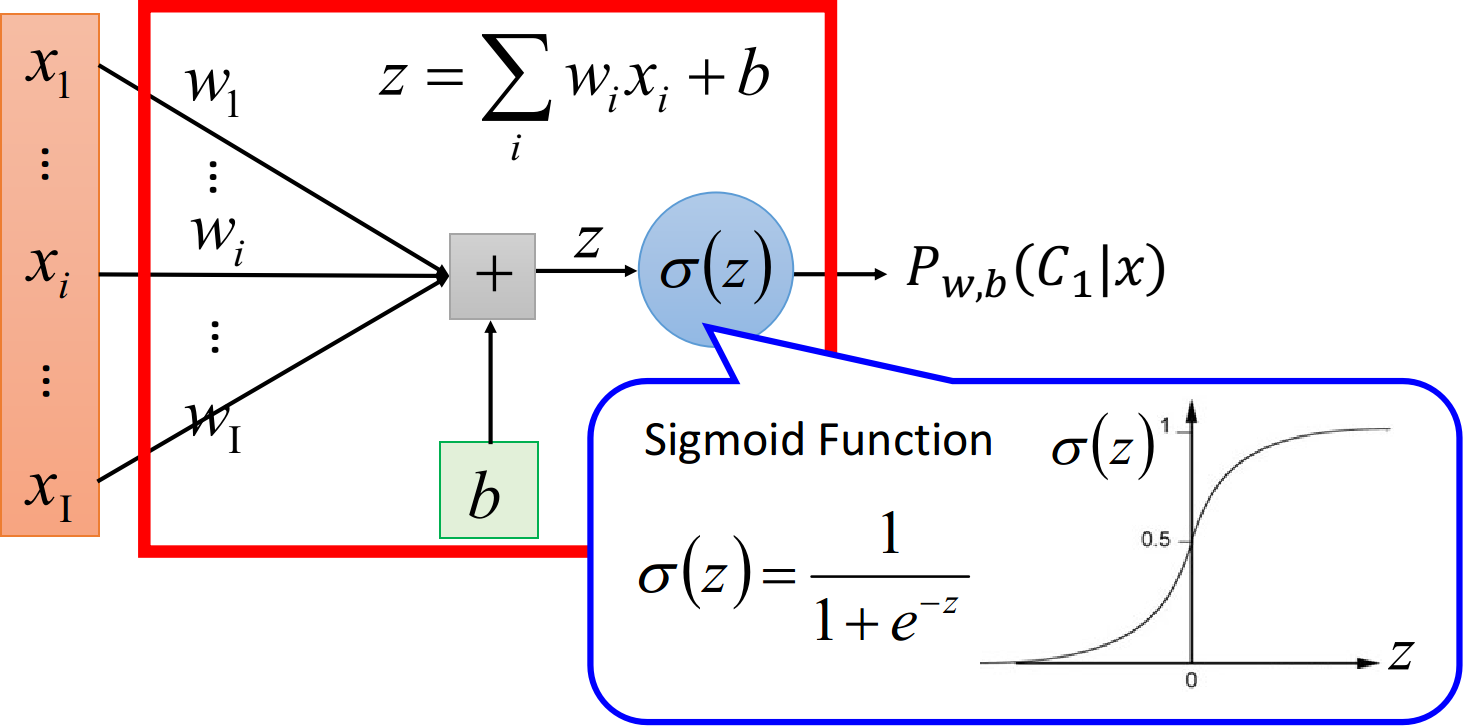
\includegraphics[width=0.5\linewidth]{LR.png}
    \caption{逻辑回归示意图}
    \label{fig:LR}
\end{figure}

假设Training data是从我们定义的Posterior Probability中产生的(后置概率,某种意义上就是概率密度函数),而w和b决定了这个Posterior Probability,此时可以去计算某一组w和b产生这N个样本点的概率,根据极大似然估计的思想,最好的那组参数就是有最大可能性产生当前N个样本点分布的$w^*$和$b^*$。最终利用极大似然估计法推导出其损失函数,并表示为交叉熵的形式如下:

\begin{equation}
    \begin{aligned}
        w^*,b^* & =\arg \max\limits_{w,b} L(w,b)                                                 \\
                & =\arg\min\limits_{w,b}(-\ln L(w,b)                                             \\
                & =\sum\limits_n -[\hat{y}^n \ln f_{w,b}(x^n)+(1-\hat{y}^n) \ln(1-f_{w,b}(x^n))]
    \end{aligned}
\end{equation}

随后计算出参数的偏导,利用梯度下降法更新参数即可:

\begin{equation}
    \begin{aligned}
        w_i=w_i-\eta \sum\limits_{n}-(\hat{y}^n-f_{w,b}(x^n))x_i^n
    \end{aligned}
\end{equation}

相比于square error, 损失函数选择cross entropy能够加快参数更新的步伐和速度,而不会导致图2中由于损失函数曲面过于平缓而停滞不前的现象

\begin{figure}[H]
    \centering
    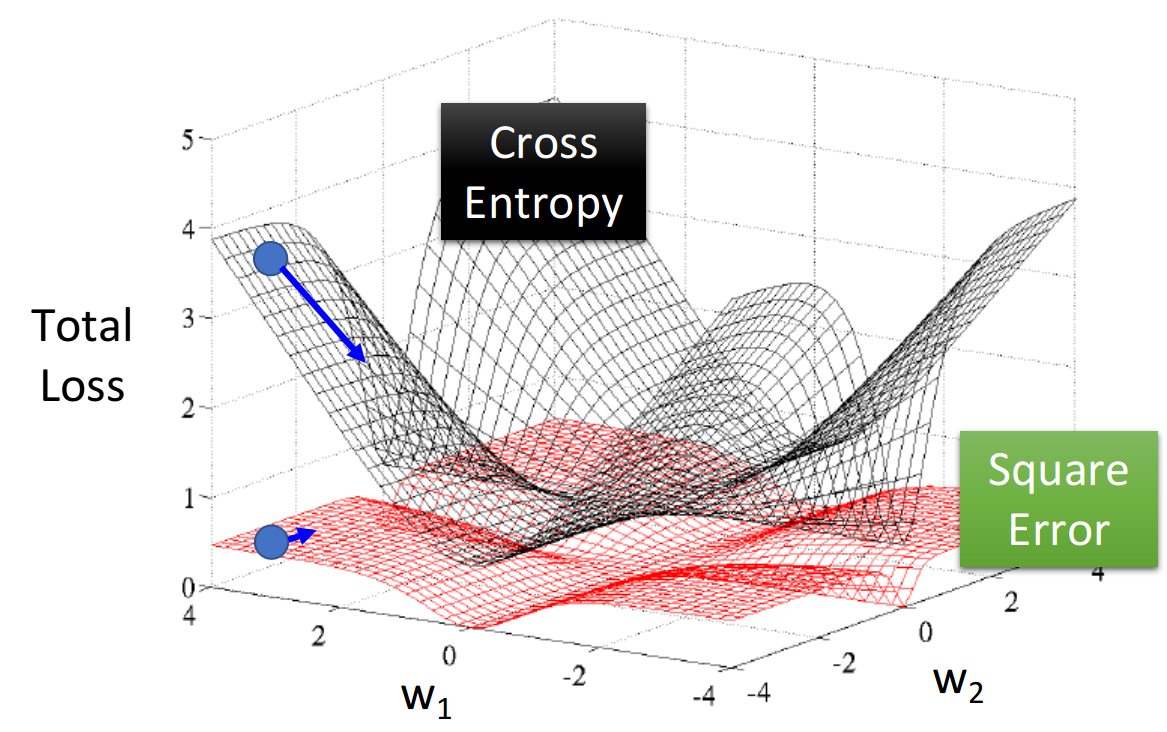
\includegraphics[width=0.5\linewidth]{ce.png}
    \caption{交叉熵vs方均根}
    \label{fig:ce}
\end{figure}

\subsubsection{逻辑回归的限制}

Logistic Regression的应用其实有不少的限制,给出图3中样本点分布,想要用逻辑回归对它进行分类,其实是做不到的。因为逻辑回归在两个class之间的boundary就是一条直线,但是在这个平面上无论怎么画直线都不可能把图中的两个class分隔开来。

\begin{figure}[H]
    \centering
    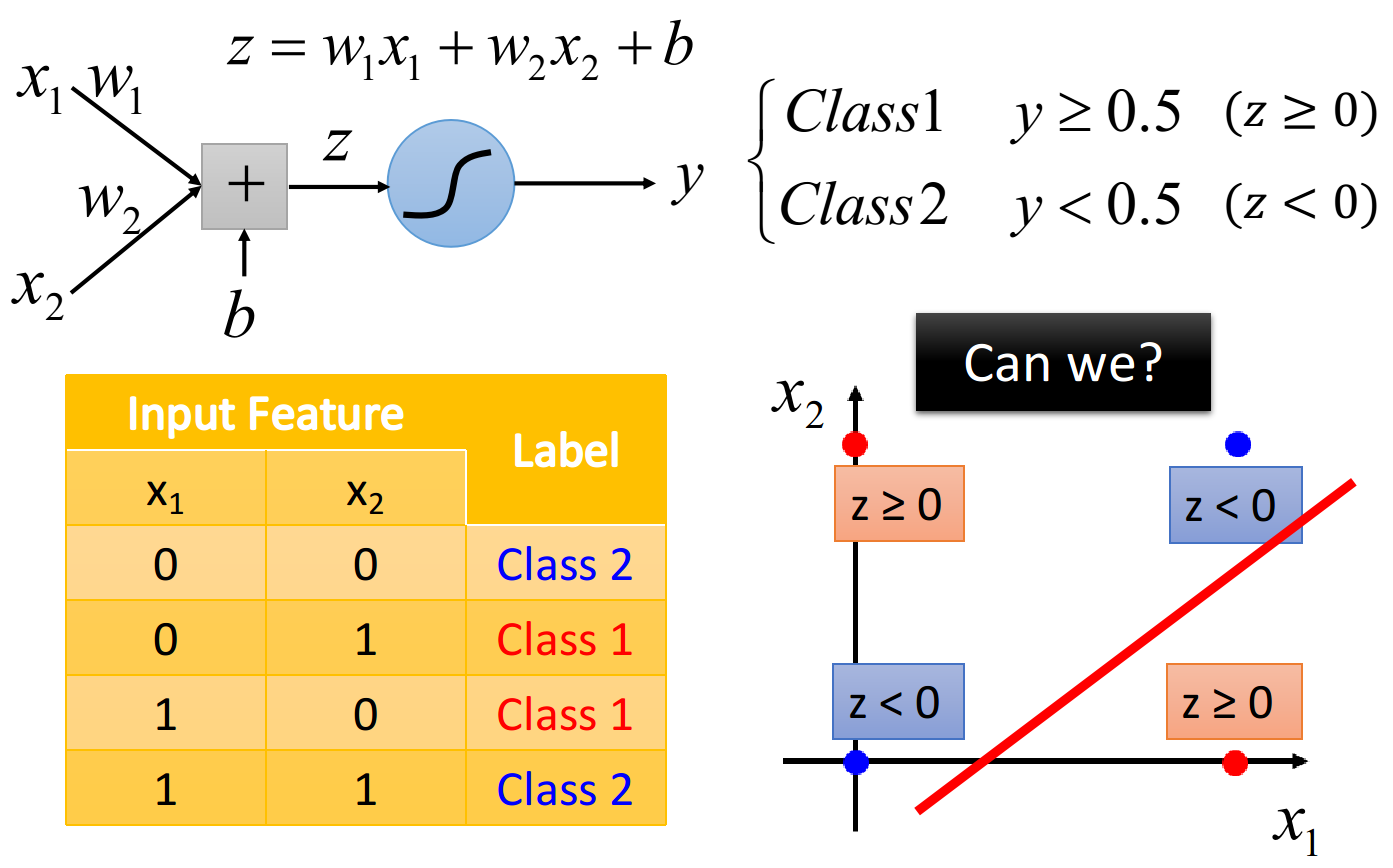
\includegraphics[width=0.6\linewidth]{limit.png}
    \caption{逻辑回归的限制}
    \label{fig:limit}
\end{figure}

如果坚持要用逻辑回归的话,可以使用Feature Transformation把原先的特征分布投影到一个比新的特征空间。\\

假设定义$x_1'$是原来的点到$\begin{bmatrix}0\\0 \end{bmatrix}$之间的距离,$x_2'$是原来的点到$\begin{bmatrix}1\\ 1 \end{bmatrix}$之间的距离,重新映射之后如图4右侧所示(红色两个点重合),此时逻辑回归就可以顺利把它们划分开来。

\begin{figure}[H]
    \centering
    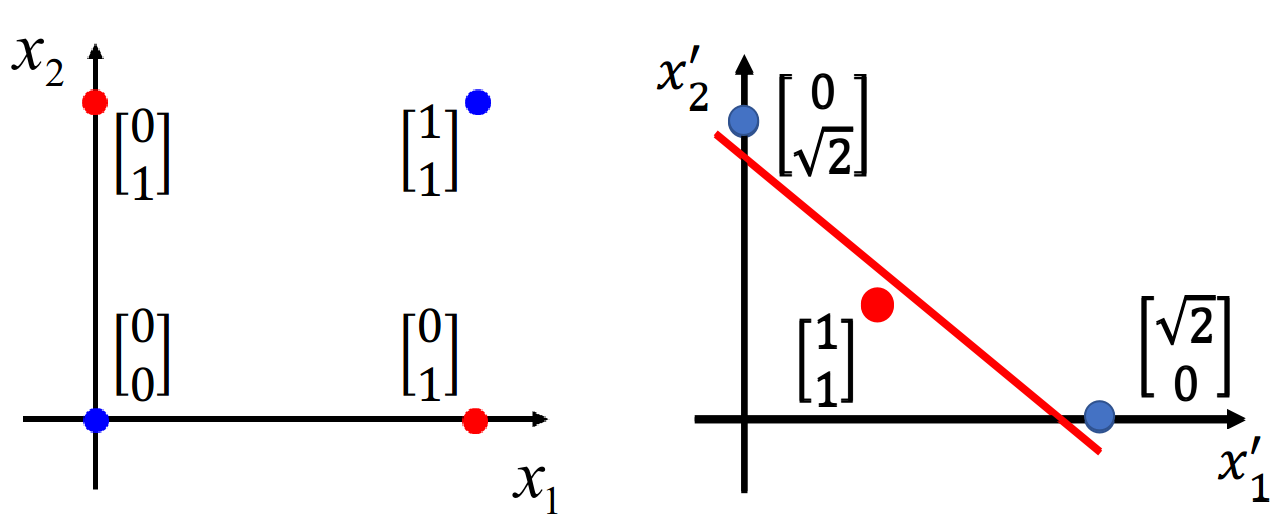
\includegraphics[width=0.6\linewidth]{transform.png}
    \caption{特征映射}
    \label{fig:transform}
\end{figure}

但实际上,如何做恰当feature Transformation本身就是个难题,如果在这上面花费太多时间就得不偿失了。\textbf{级联逻辑回归}的提出解决了这个问题,先用n个逻辑回归做特征转换,再用1个逻辑回归作为新特征的分类器,它们的参数都可以通过梯度下降来得到。

\subsubsection{级联逻辑回归到神经网络}
在级联逻辑回归中,如果把每一个逻辑回归叫做一个neuron(神经元),把这些用于feature Transformation的逻辑回归串联起来所形成的网络,叫做Neural Network(神经网络),那么级联逻辑回归就是我们所熟知的深度学习神经网络模型,sigmoid函数则是每个神经元的激活函数。

\begin{figure}[H]
    \centering
    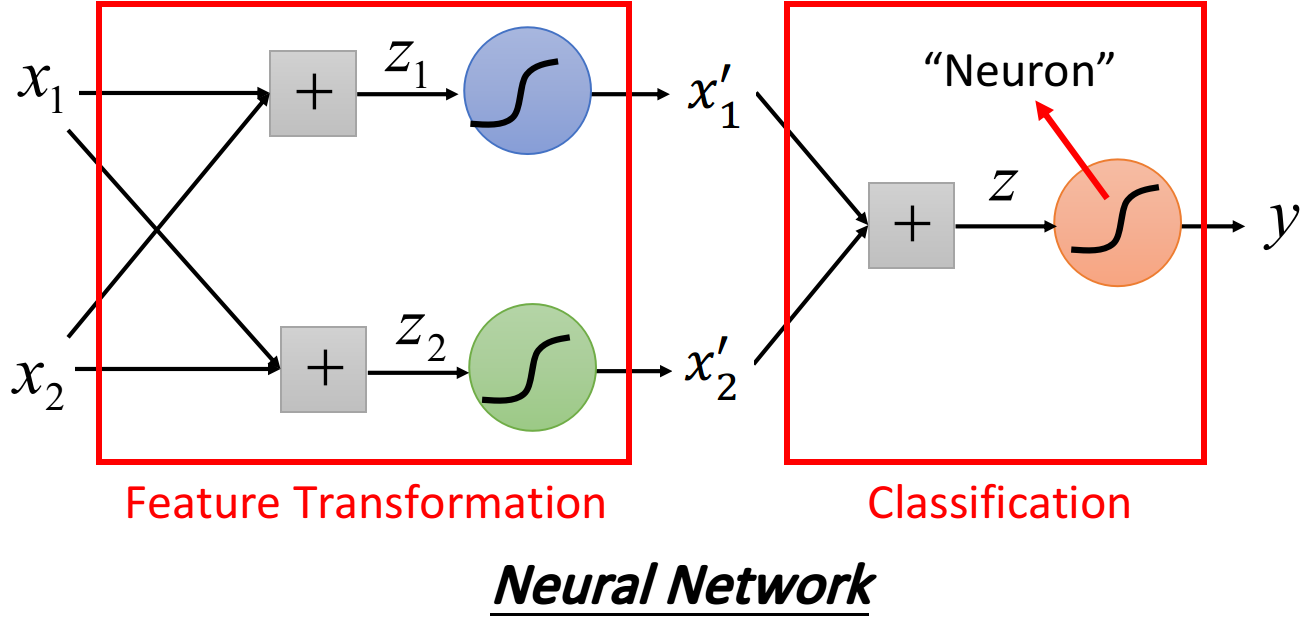
\includegraphics[width=0.8\linewidth]{nn.png}
    \caption{级联逻辑回归即神经网络模型}
    \label{fig:nn}
\end{figure}

\subsection{从神经网络到自编码器}
\subsubsection{神经网络的本质}
从前面的推导可以看出,神经网络的众多隐藏层本质上就是一个个特征提取器,随着网络层数的增加,检测的特征从简单变为复杂,最终通过后续的输出层分类器,得到分类的结果。\\

如果直接用神经网络作为分类器,也可以得到较好的分类效果。虽然神经网络的特征提取能力是毋庸置疑的,但在整个网络架构中,作为分类器部分的后几层layer并不一定能够得到充分的训练,导致分类准确率无法得到进一步的提升。\\

而本文的创新点在于,用随机森林、LightGBM等树模型作为神经网络后半部分的分类器。换一种说法就是,并不直接用神经网络作为分类器,而是\textbf{把神经网络提取到的特征用于训练其他更专业更高性能的分类模型}。实际操作上就是把神经网络隐藏层的输出接到其他分类模型的输入上,以期得到更好的分类效果。

\subsubsection{自编码器提取隐藏层输出}
如何获取隐藏层输出呢?自编码器(Auto-encoder)提供了一种很好的思路,它的基本思想是,通过神经网络将原先的高维特征投影到非线性的低维空间上,并通过同样的网络结构重新映射回原先的空间,利用还原前后样本特征之间的差异作为损失函数,直到可以实现稳定特征转换为止。

\begin{figure}[H]
    \centering
    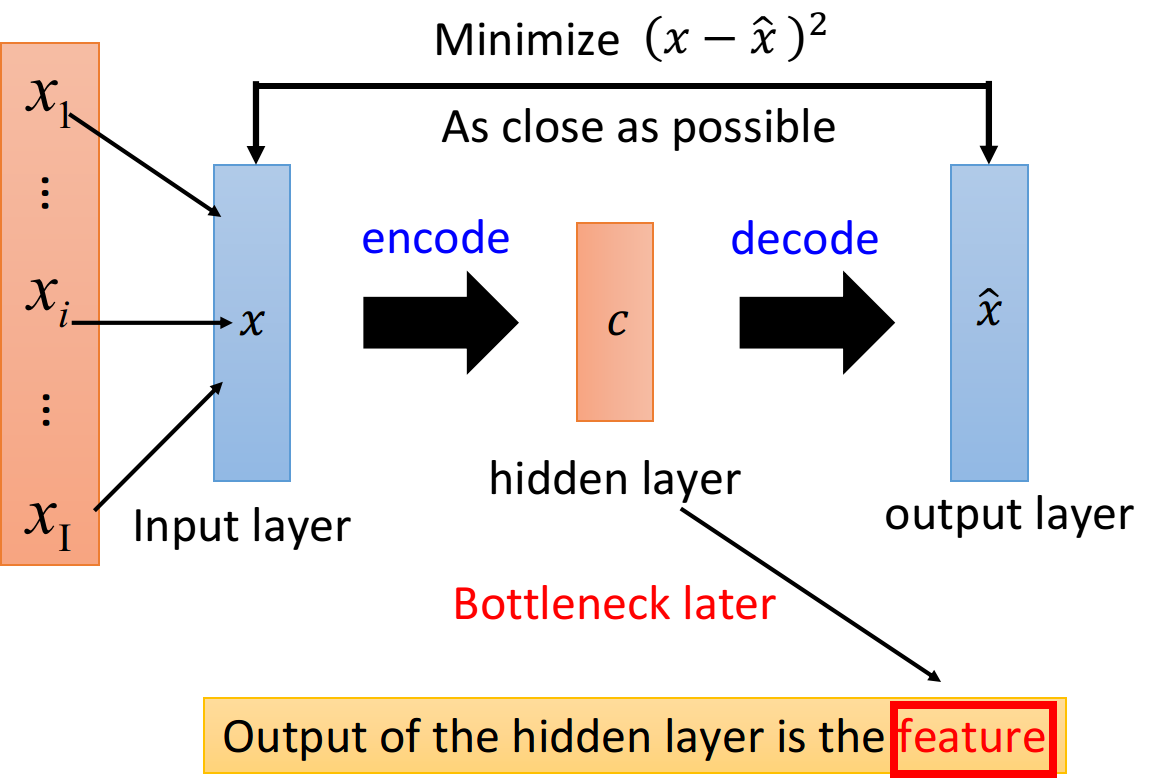
\includegraphics[width=0.6\linewidth]{autoencoder.png}
    \caption{自编码器提取特征}
    \label{fig:autoencoder}
\end{figure}

从图6中可以看出,中间hidden layer的输出就是我们希望通过神经网络提取到的特征,接下来用这些特征去训练随机森林、LightGBM等树模型,或是重新丢给一个神经网络分类器,来获取最终的分类结果。

\subsection{分类模型简介}
获取到新的特征之后,最终还是需要用专业的分类模型来划分样本点,本文主要使用随机森林、LightGBM、逻辑回归、DNN分类器来作为进一步的分类模型。这里将简要介绍随机森林和LightGBM这两个树模型。

\subsubsection{随机森林}
随机森林是一种集成算法(Ensemble Learning),它属于Bagging类型,通过组合多个弱分类器,最终结果通过投票或取均值,使得整体模型的结果具有较高的精确度和泛化性能。\\

Bagging也叫自举汇聚法(bootstrap aggregating),是一种在原始数据集上通过有放回抽样重新选出k个新数据集来训练分类器的集成技术。它使用训练出来的分类器的集合来对新样本进行分类,然后用多数投票或者对输出求均值的方法统计所有分类器的分类结果,结果最高的类别即为最终标签。此类算法可以有效降低bias,并能够降低variance。

\begin{figure}[H]
    \centering
    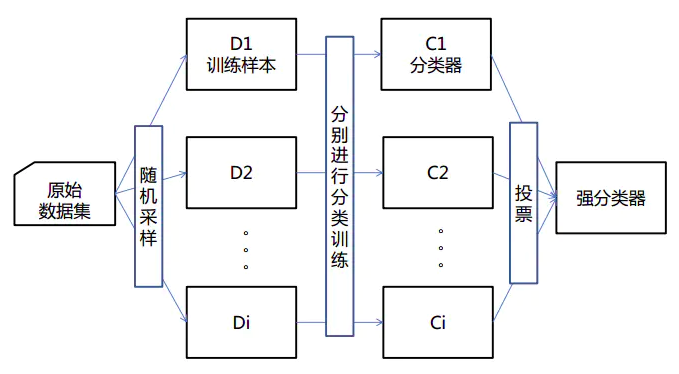
\includegraphics[width=0.6\linewidth]{rf.png}
    \caption{随机森林示意图}
    \label{fig:rf}
\end{figure}

随机森林的基本特性如下:
\begin{itemize}
    \item RF使用了CART决策树作为弱学习器
    \item 在生成每棵树的时候,每个树选取的特征都仅仅是随机选出的少数特征,一般默认取特征总数m的开方
    \item 相对于一般的Bagging算法,RF会选择采集和训练集样本数N一样个数的样本
    \item 由于随机性,对于降低模型的方差很有作用,故随机森林一般不需要额外做剪枝,即可以取得较好的泛化能力和抗过拟合能力
\end{itemize}

\subsubsection{LightGBM}
GBDT (Gradient Boosting Decision Tree) 是最常见的分类模型之一,其主要思想是利用弱分类器(决策树)迭代训练以得到最优模型,具有训练效果好、不易过拟合等优点。LightGBM (Light Gradient Boosting Machine)则是一个实现 GBDT 算法的框架,支持高效率的并行训练,并且具有以下优点:
\begin{itemize}
    \item 更快的训练速度
    \item 更低的内存消耗
    \item 更好的准确率
    \item 分布式支持,可以快速处理海量数据
\end{itemize}

GBDT在每一次迭代的时候,都需要遍历整个训练数据多次,导致训练效率低下,而LightGBM则针对这一情况做了优化,变得更轻量。它使用了基于 Histogram的决策树算法,根据直方图的离散值,遍历寻找最优的分割点。此外,它抛弃了大多数 GBDT 工具使用的按层生长 (level-wise) 的决策树生长策略,而使用了带有深度限制的按叶子生长 (leaf-wise) 算法。\\

Leaf-wise 是一种更为高效的策略,每次从当前所有叶子中,找到分裂增益最大的一个叶子,然后分裂,如此循环。同GDBT使用的 Level-wise 策略相比,在分裂次数相同的情况下,Leaf-wise 可以降低更多的误差,得到更好的精度。Leaf-wise 的缺点是可能会长出比较深的决策树,产生过拟合。因此 LightGBM 在 Leaf-wise 之上增加了一个最大深度的限制,在保证高效率的同时防止过拟合。\\

LightGBM 还具有支持高效并行的优点。LightGBM 原生支持并行学习,目前支持特征并行和数据并行的两种,并且针对这两种并行方法都做了优化。\\



\newpage
\section{数据集分析}
\subsection{分析方法概述}
对于数据集的分析,本文主要采用了EDA(Exploratory Data Analysis)的思想。\\
EDA是一种采用各种方法(主要指数据迹线、直方图、概率图等图形化方法)的数据分析方法。EDA的优势主要包括:
\begin{itemize}
	\item 最大限度地洞察数据集
	\item 揭示底层结构
	\item 提取重要变量
	\item 检测异常值
	\item 测试基本假设
	\item 建立初步模型
	\item 确定最佳因子设置
\end{itemize}
本章初步分析了题目数据集,了解数据集特征的同时也完成了传统的数据清洗、特征工程环节。便于后续和本文提出的新模型进行分析对比。
\subsection{具体分析}
通过查看好坏比、缺失值、相关度矩阵,初步确定数据集存在不平衡、缺失值和噪声等,需要清洗。
本节挑选具有代表性的属性进行分析。其他属性采用类似的分析方法,故不赘述。
\subsubsection{Age}
\begin{itemize}
	\item 查看数据分布情况
	      \begin{figure}[H]
		      \centering
		      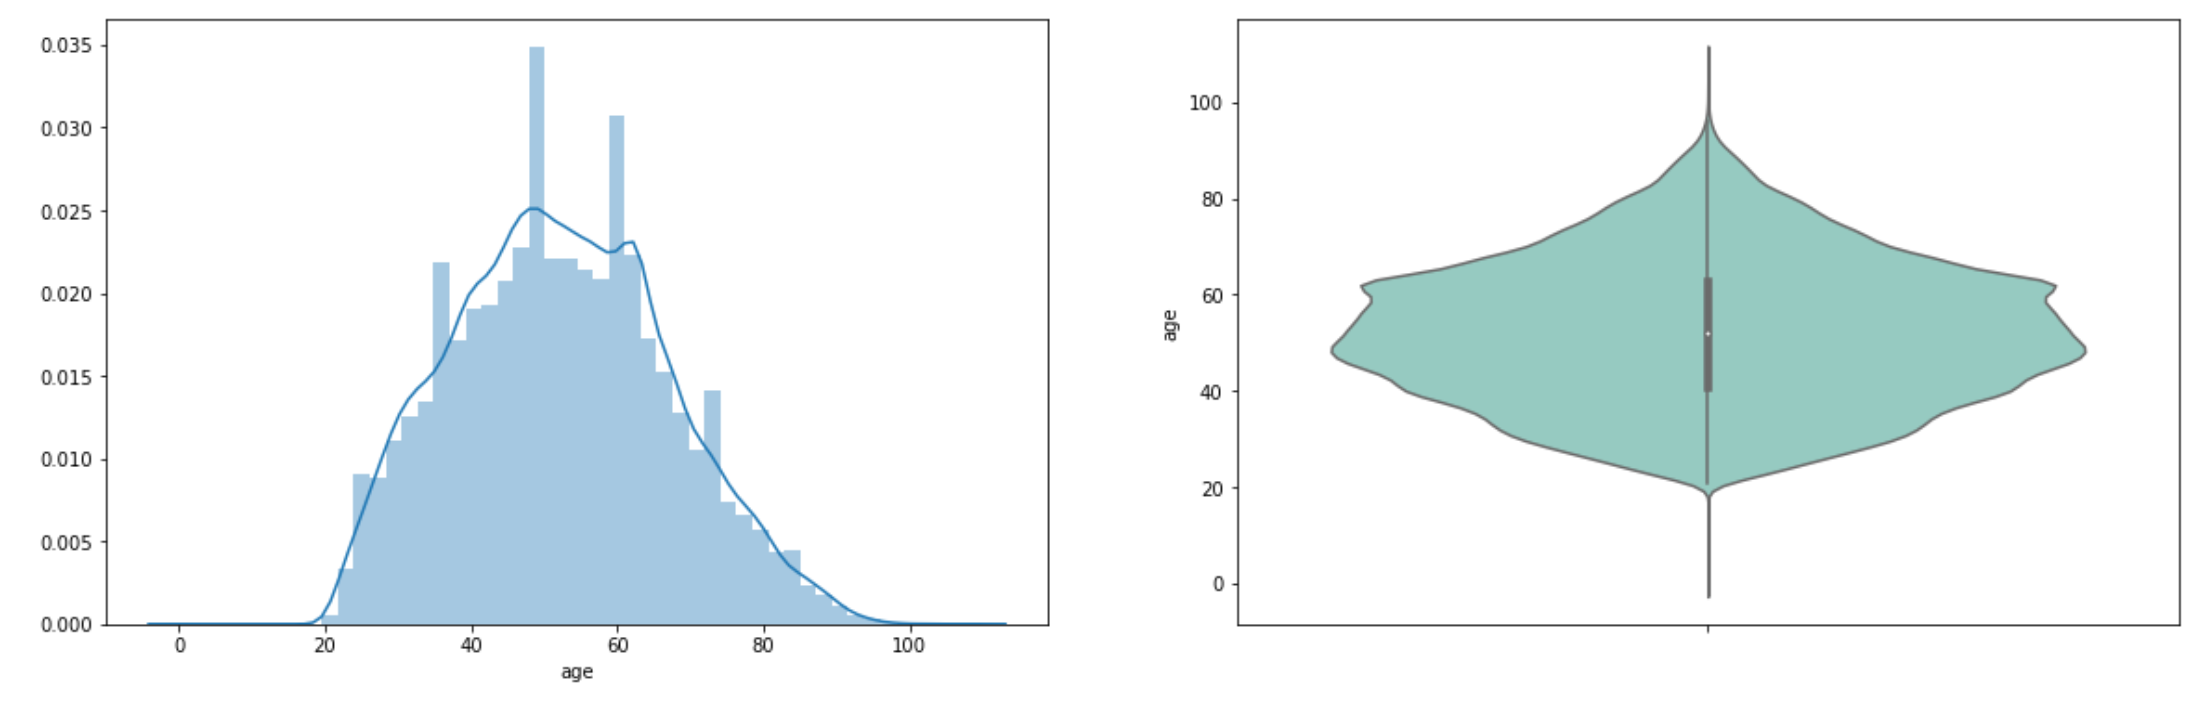
\includegraphics[width=1.0\linewidth]{age_distribution.png}
		      \caption{Age的分布情况}
	      \end{figure}
	      可见数据大致符合正态分布,存在一定噪声。同时由于年龄属性的特殊性,后续的数据清洗工作中需要估计年龄的上下界,以便更好消噪。
	\item 利用直方图查看age和预测值间的关系
	      \begin{figure}[H]
		      \centering
		      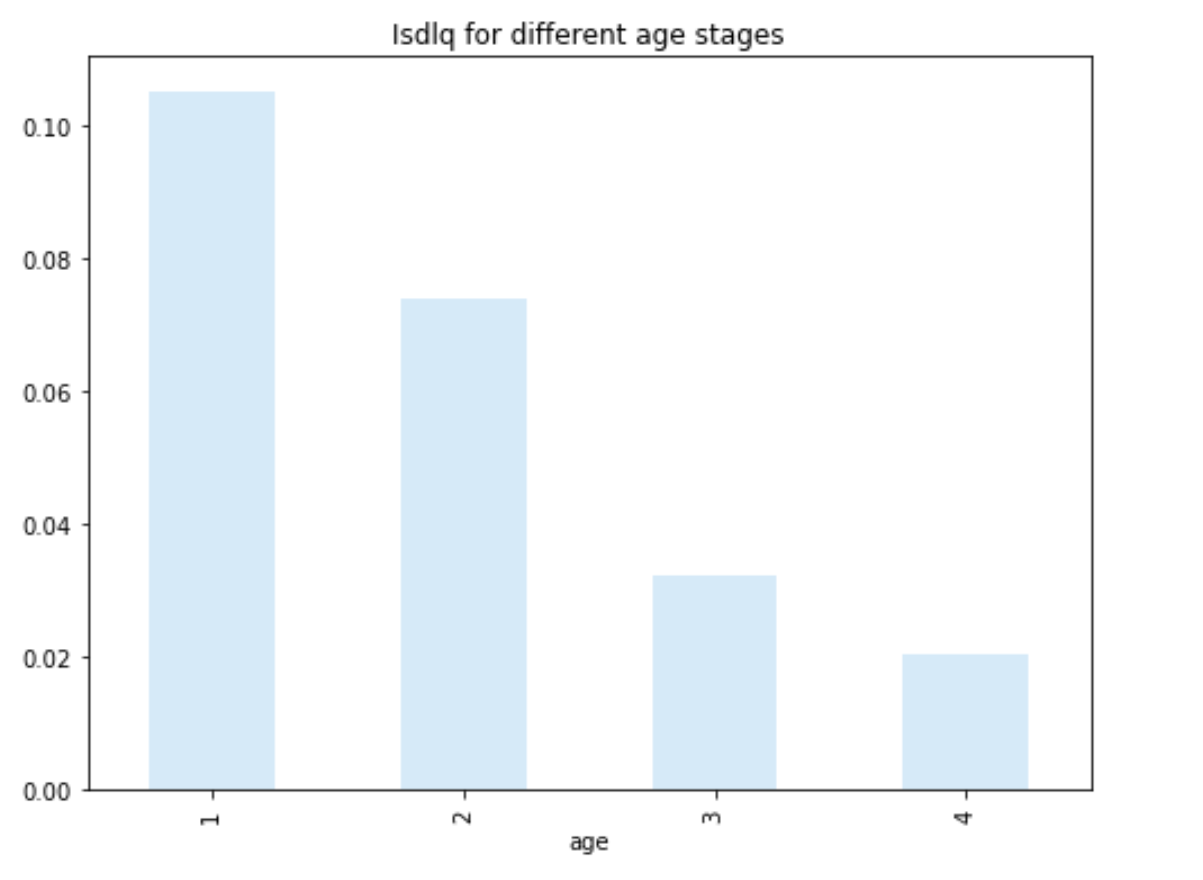
\includegraphics[width=0.8\linewidth]{age_histogram.png}
		      \caption{Age和Isdlq的关系}
	      \end{figure}
	      可见违约率随年龄递减。
	      \subsubsection{Revol}
	\item 查看数据分布情况
	      \begin{figure}[H]
		      \centering
		      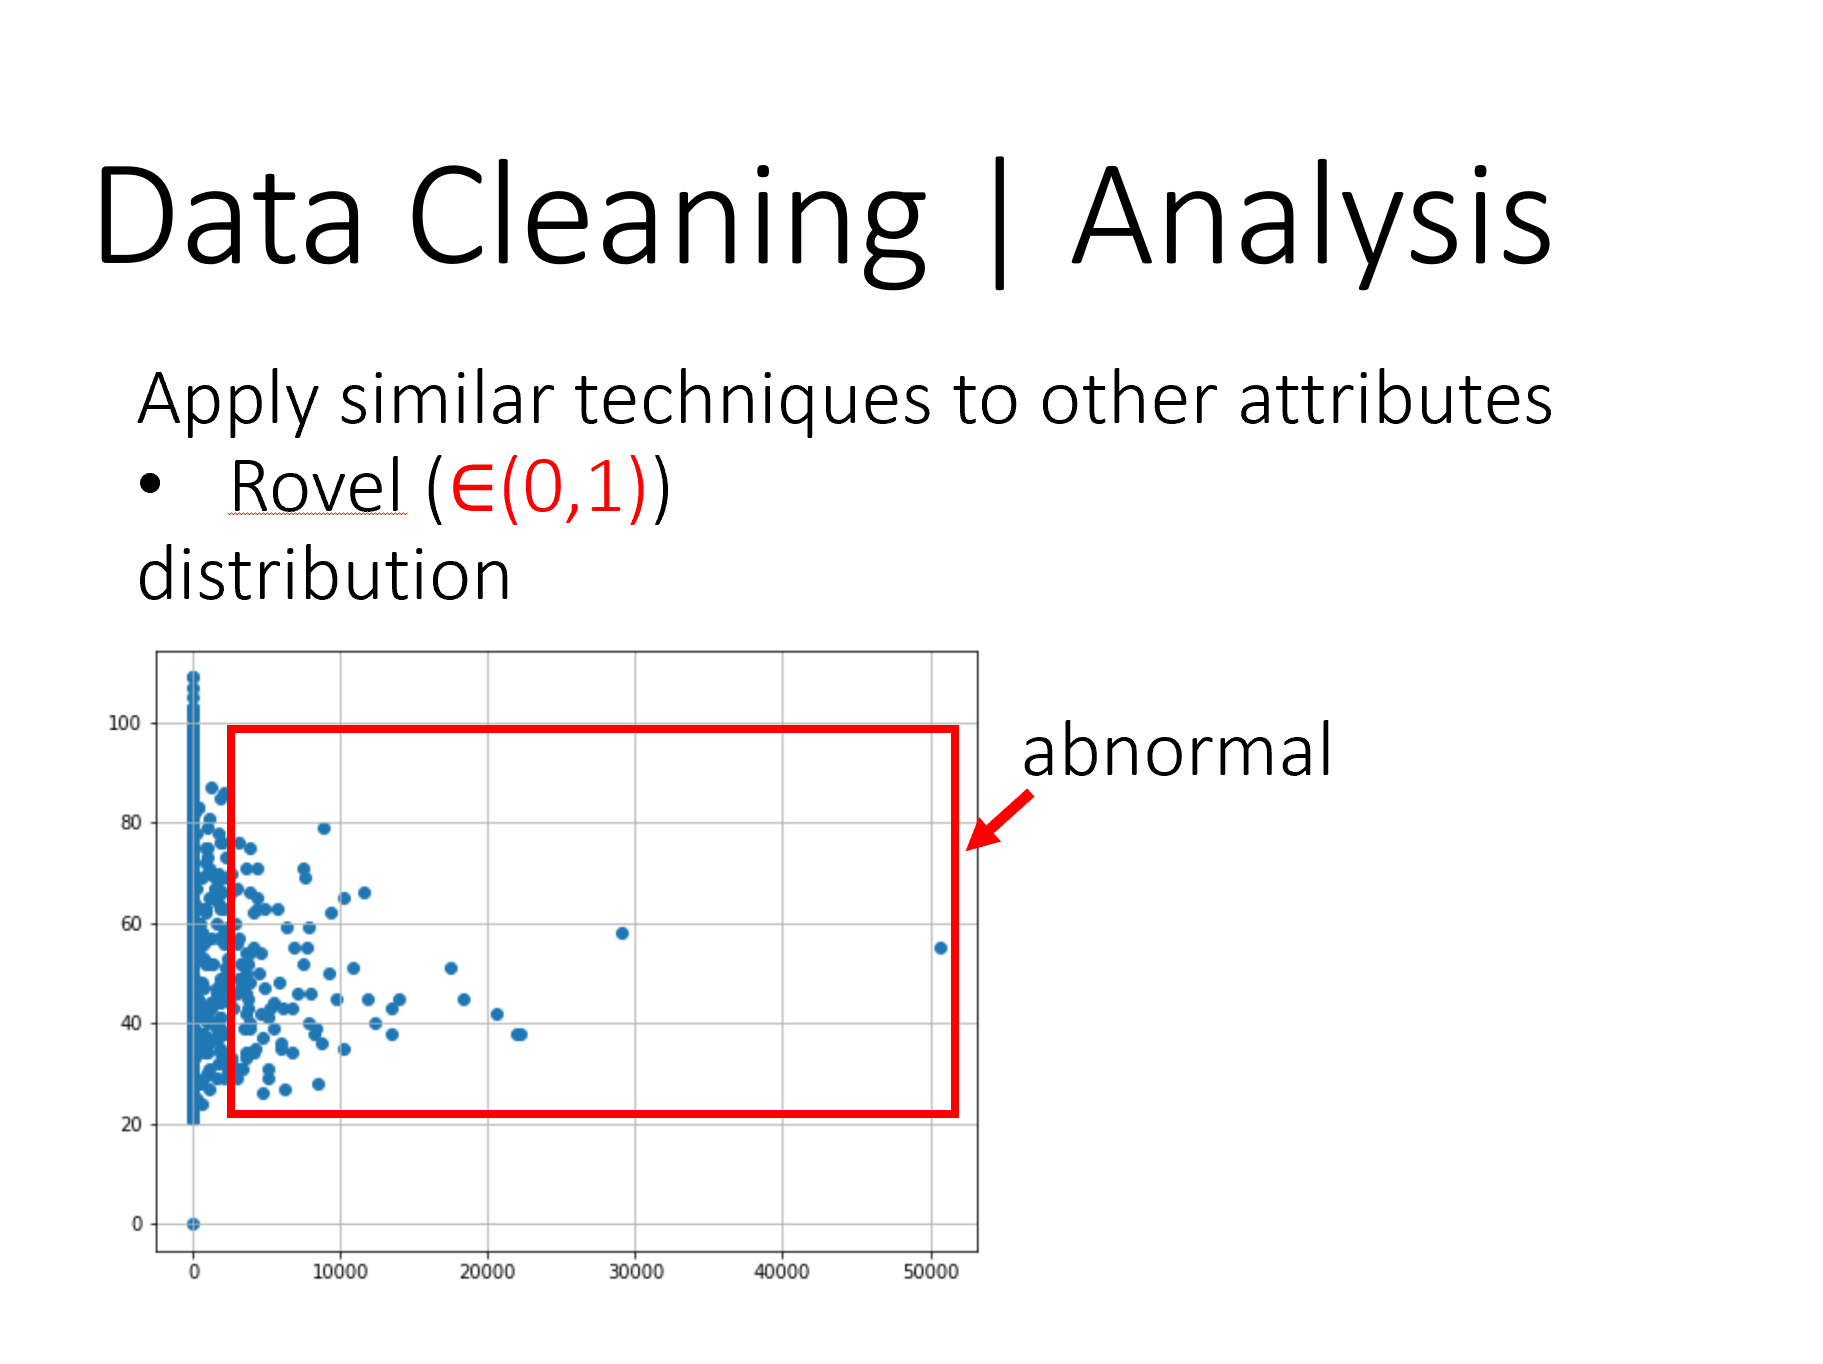
\includegraphics[width=0.6\linewidth]{revol_distribution.png}
		      \caption{Revol的分布情况}
		      \label{fig:rd}
	      \end{figure}
	      值得注意的是,Revol的合理区间应该是[0,1],而数据中却出现了明显的异常值。异常值可能来自于噪声,也可能来自于未规约化的正常数据。为了更大程度利用数据,本文继续查看了不同scale的数据直方图,大致确定可以舍去的异常值的范围。
	\item 利用不同scale直方图估计异常值区间
	      \begin{figure}[H]
		      \centering
		      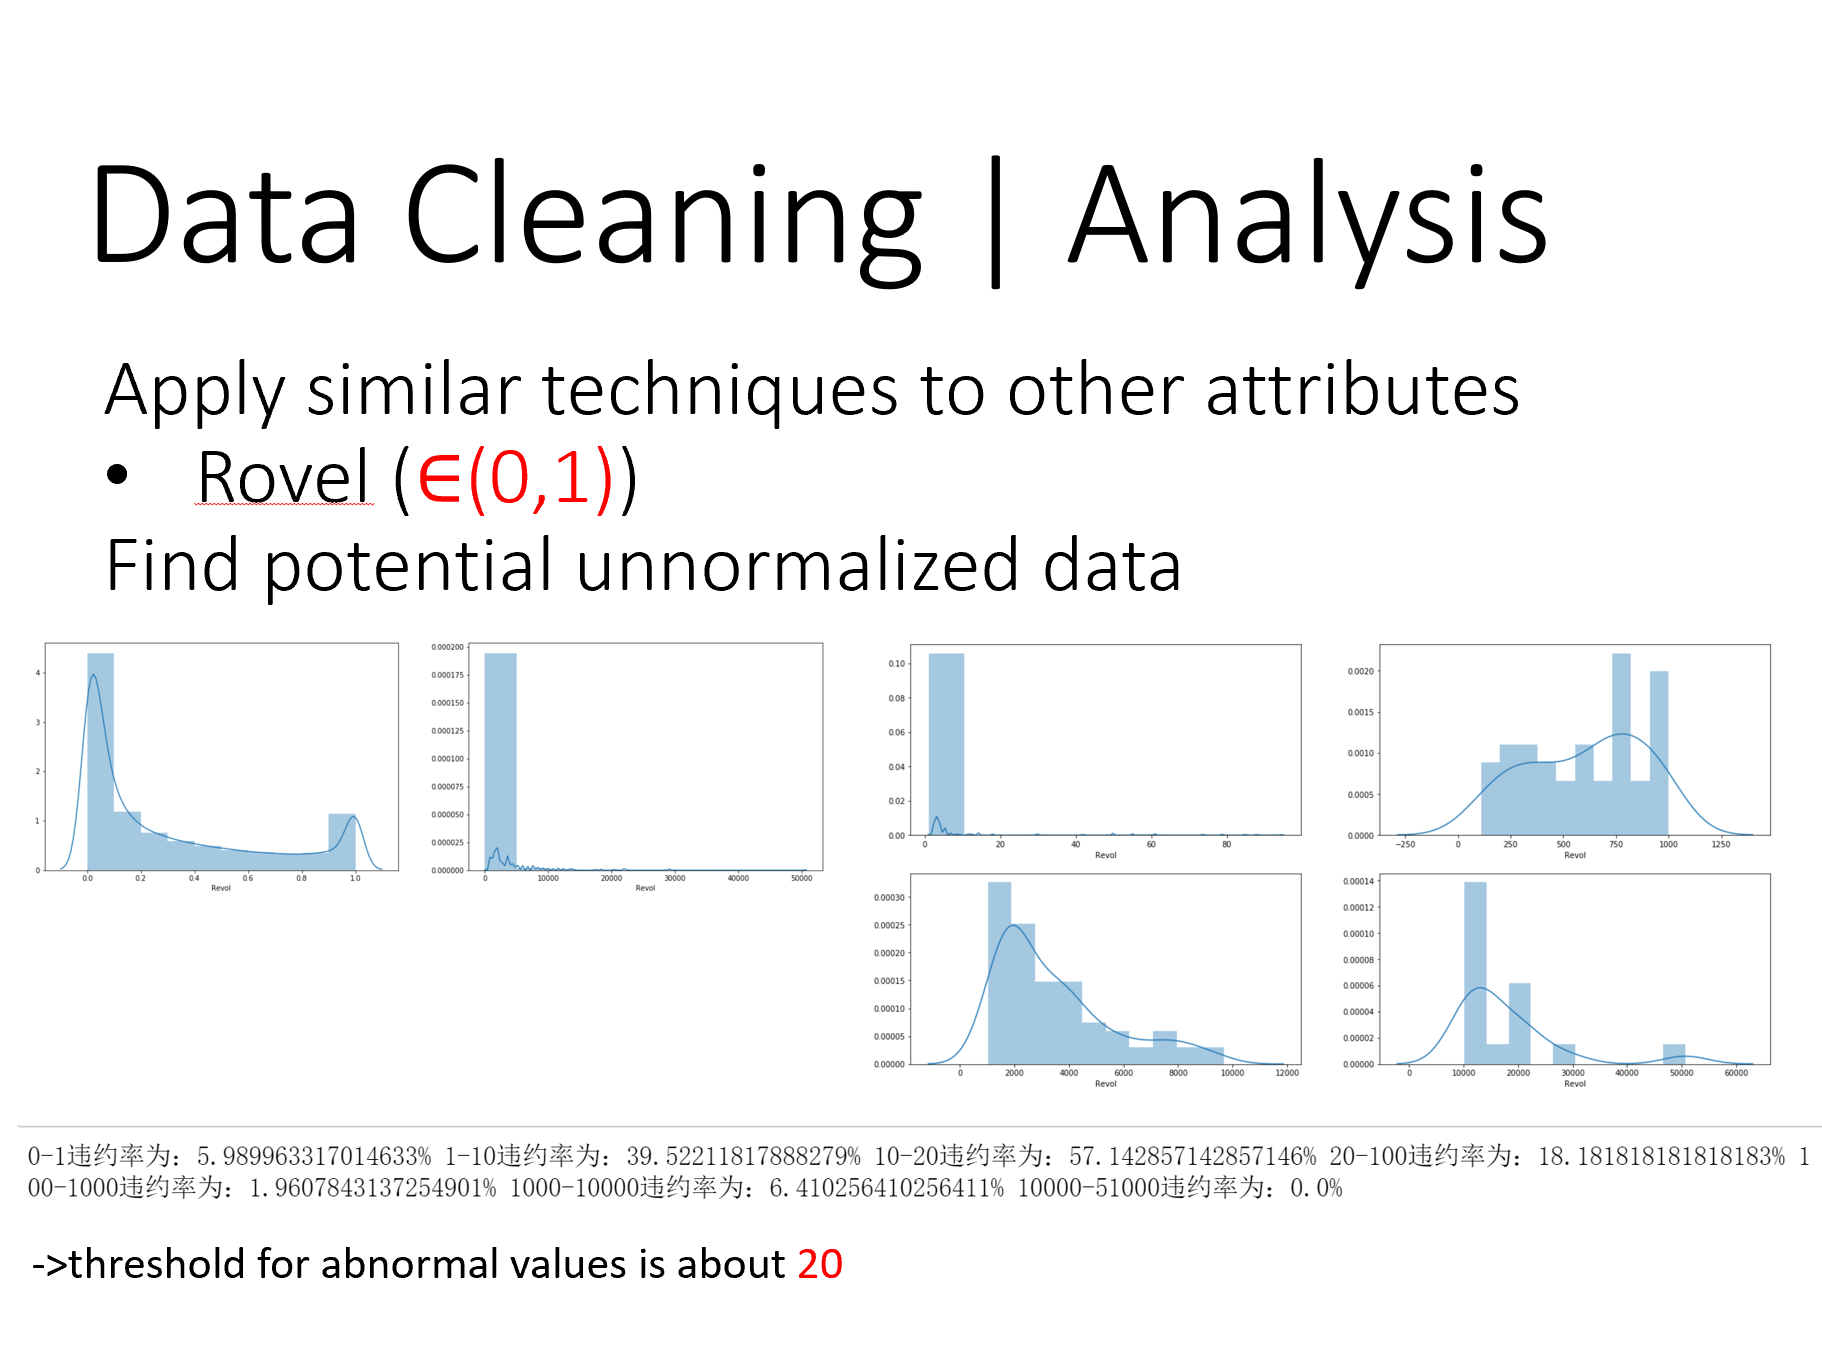
\includegraphics[width=0.6\linewidth]{revol_find_bounds.png}
		      \caption{不同区间的Revol直方图}
		      \label{fig:rh}
	      \end{figure}
	      因数据分布跨度比较大,我们将数据分为两部分,小于1和大于1的部分。\\
	      可以看出在Revol大于1时,违约率开始上升,10-20之间违约率达到高峰,超过20后开始下降,超过1000后开始恢复正常(与0-1的违约率一致),说明20左右的值可能为异常值上限的阈值。可以将超过20的值都定义为异常值。     
\end{itemize}

\subsection{数据清洗}
根据EDA分析中得出的结论。对数据集进行清洗,本文采用的具体方法包括异常值处理,缺失值填补,特征交叉衍生,数据类型转换、分箱等。
\begin{figure}[H]
	\centering
	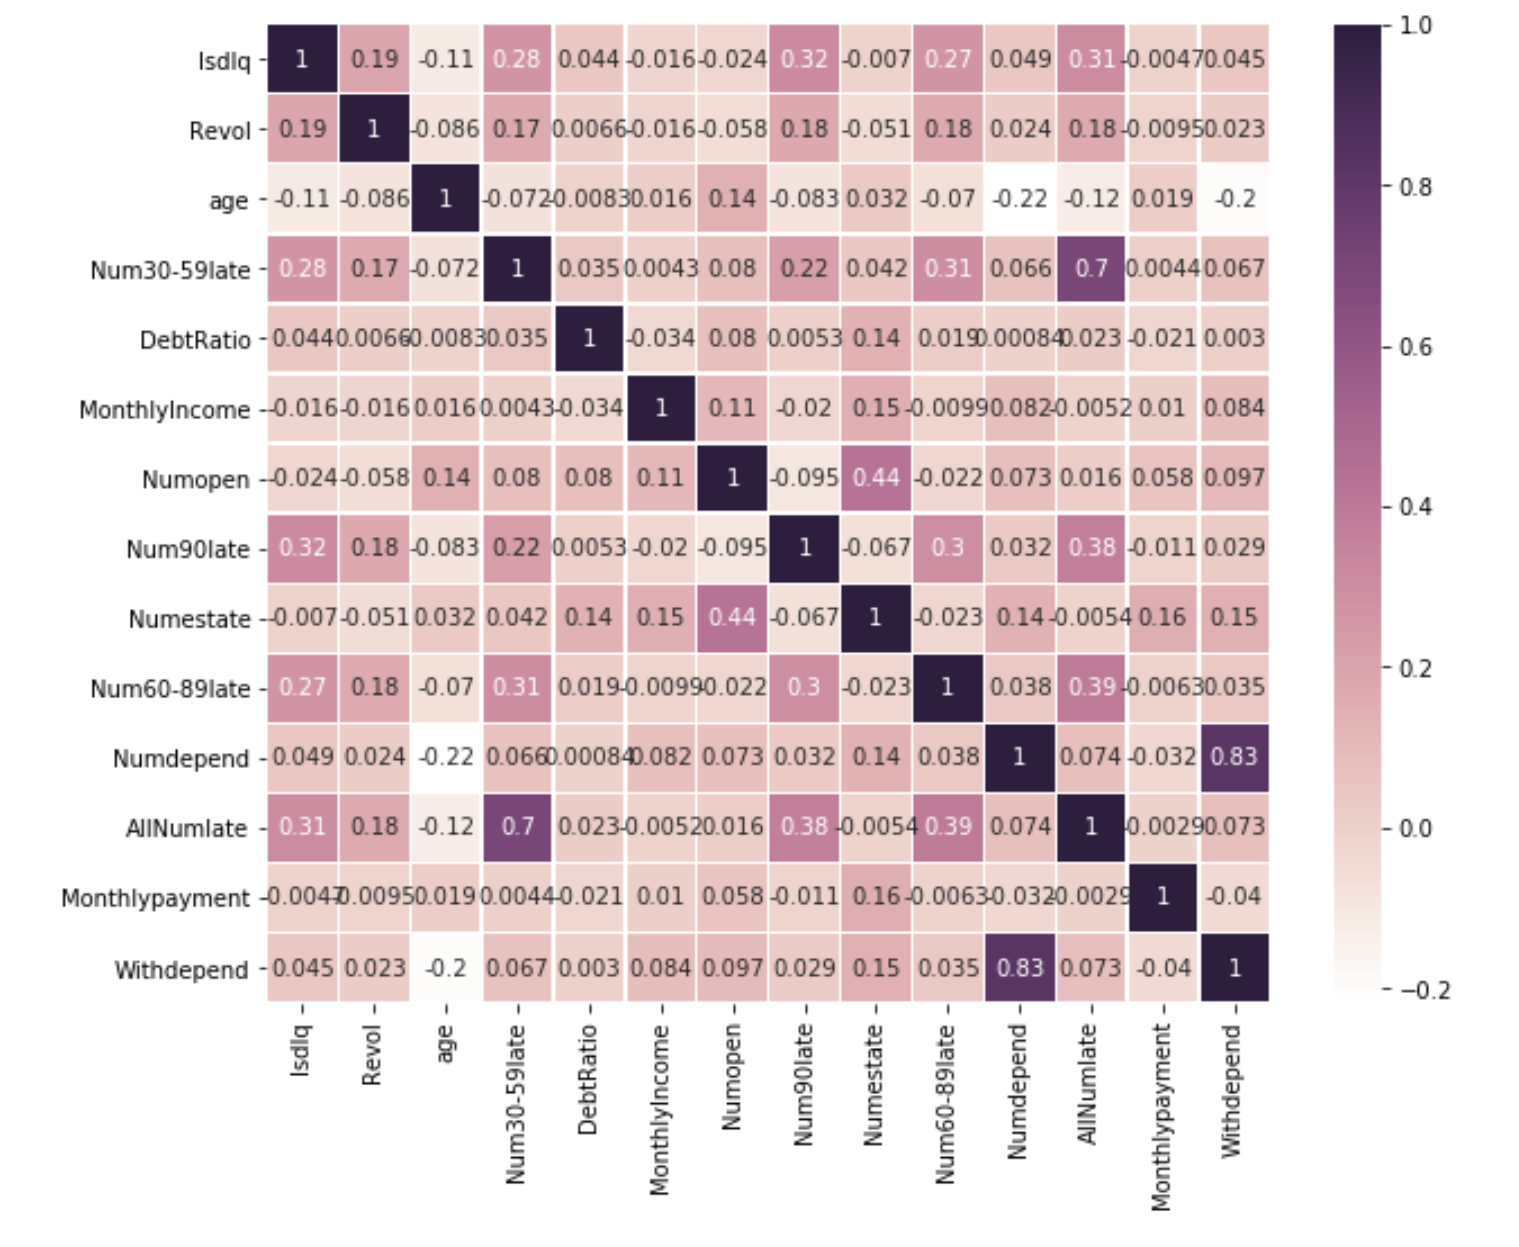
\includegraphics[width=0.8\linewidth]{heatmap.png}
	\caption{初步清洗后的相关度矩阵热力图}
	\label{fig:hm}
\end{figure}
其中,相关系数绝对值和两个变量关联程度成正比。

\subsection{特征筛选}
计算每个属性的WOE、IV值,如下图所示:
\begin{figure}[H]
	\centering
	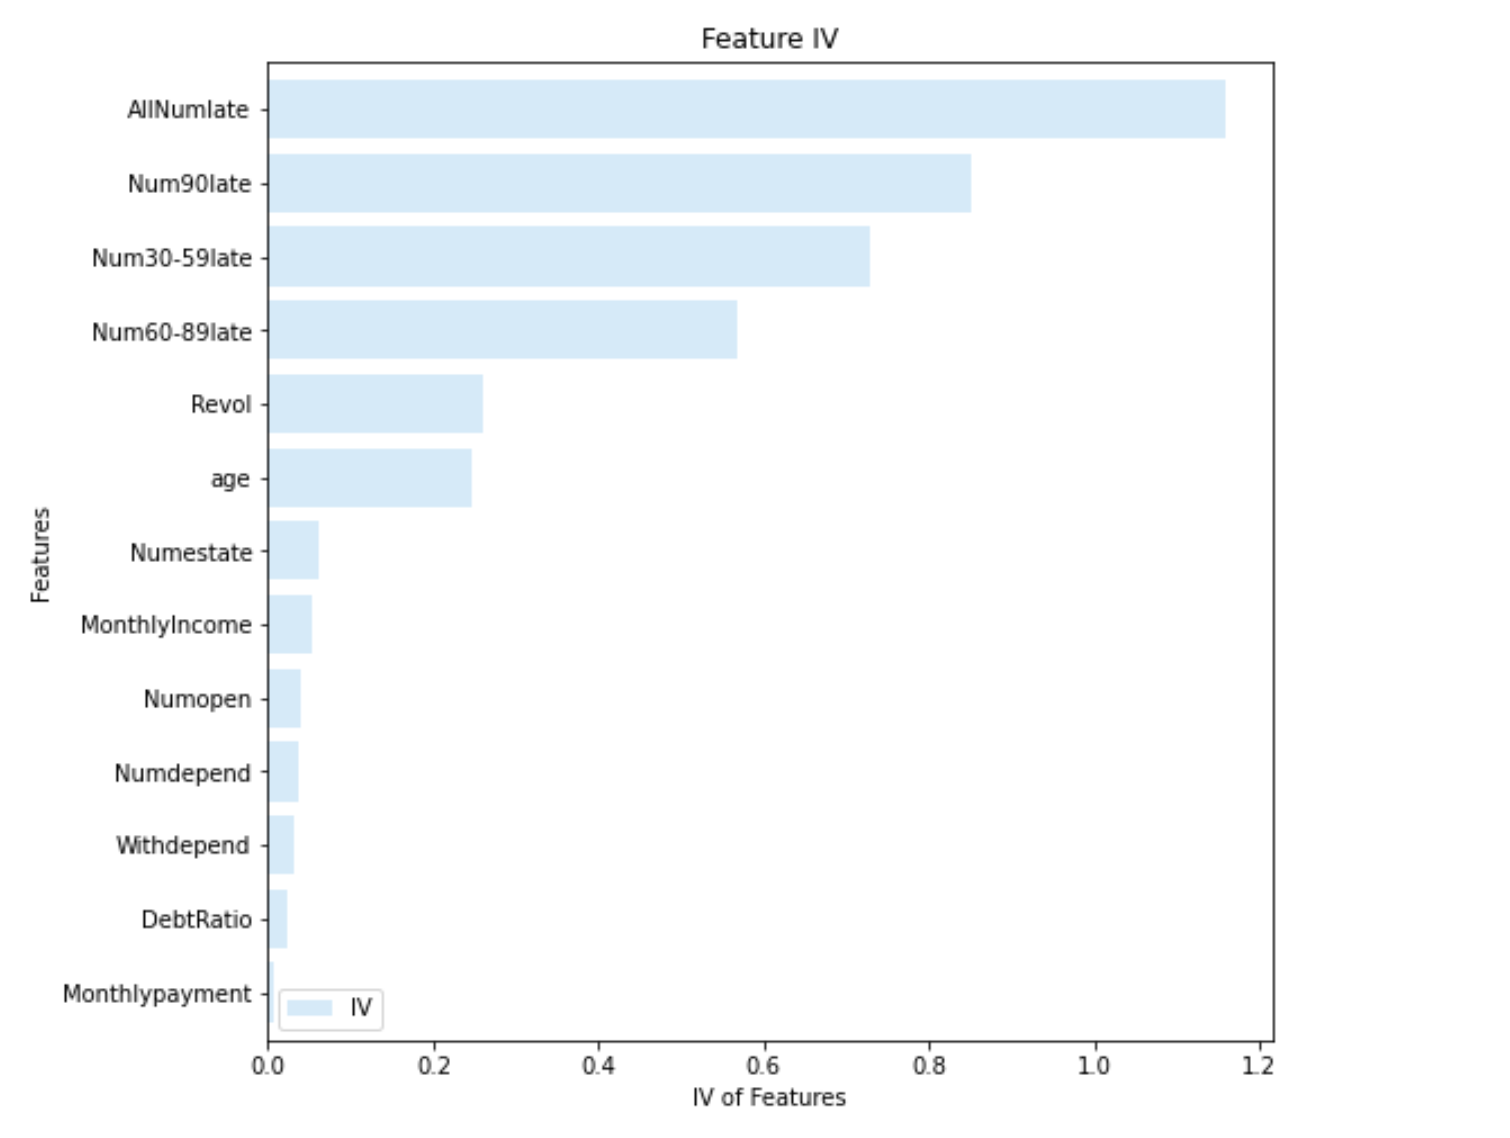
\includegraphics[width=0.8\linewidth]{IV.png}
	\caption{各属性IV值}
	\label{fig:iv}
\end{figure}

首先筛选出IV值大于0.1的变量:'Num30-59late','Num60-89late','Num90late','AllNumlate','Revol','age'。\\

从热力图看出,'Num30-59late'与'AllNumlate'具有强相关性(0.7),说明两者表征的信息具有较大的重叠,可以删掉一个。最终,两者取IV值较高者'AllNumlate'。
清洗后,最终选用特征 ['Num60-89late','Num90late','AllNumlate','Revol','age']。







\newpage
\section{实验与分析}
\subsection{实验设计说明}
为了验证本文提出的基于自编码降维的特征工程对最终分类结果的实际有效性,整个实验设计将分别使用两份数据集,并在相同参数的模型上分别进行验证和对比:

\begin{itemize}
    \item 使用常见的WOE编码、IV值筛选、特征交叉组合的特征工程处理之后的数据集
    \item 经过简单处理和WOE编码后,再利用神经网络自编码器(Auto-Encoder)进行非线性降维和特征提取后的数据集
\end{itemize}

\subsection{实验模型介绍}
如下图所示,本文采用的模型基本思路为:先通过初步特征工程和WOE编码,得到13个基本特征$x$;将这13个基本特征输入Auto-encoder神经网络模型,分别进行13维$\rightarrow$3维的特征压缩和3维$\rightarrow$13维的特征还原,还原后的结果记为$\hat x$\\

将还原前后的$x$和$\hat x$之间的差距作为神经网络的损失函数,即$Loss = \sum\limits_i (x_i-\hat x_i)^2$,对损失函数进行梯度下降,训练出一个能够稳定将13维特征压缩到3维特征的神经网络自编码器。最后,提取出隐藏层的3维特征,作为特征工程的最终结果。

\begin{figure}[H]
    \centering
    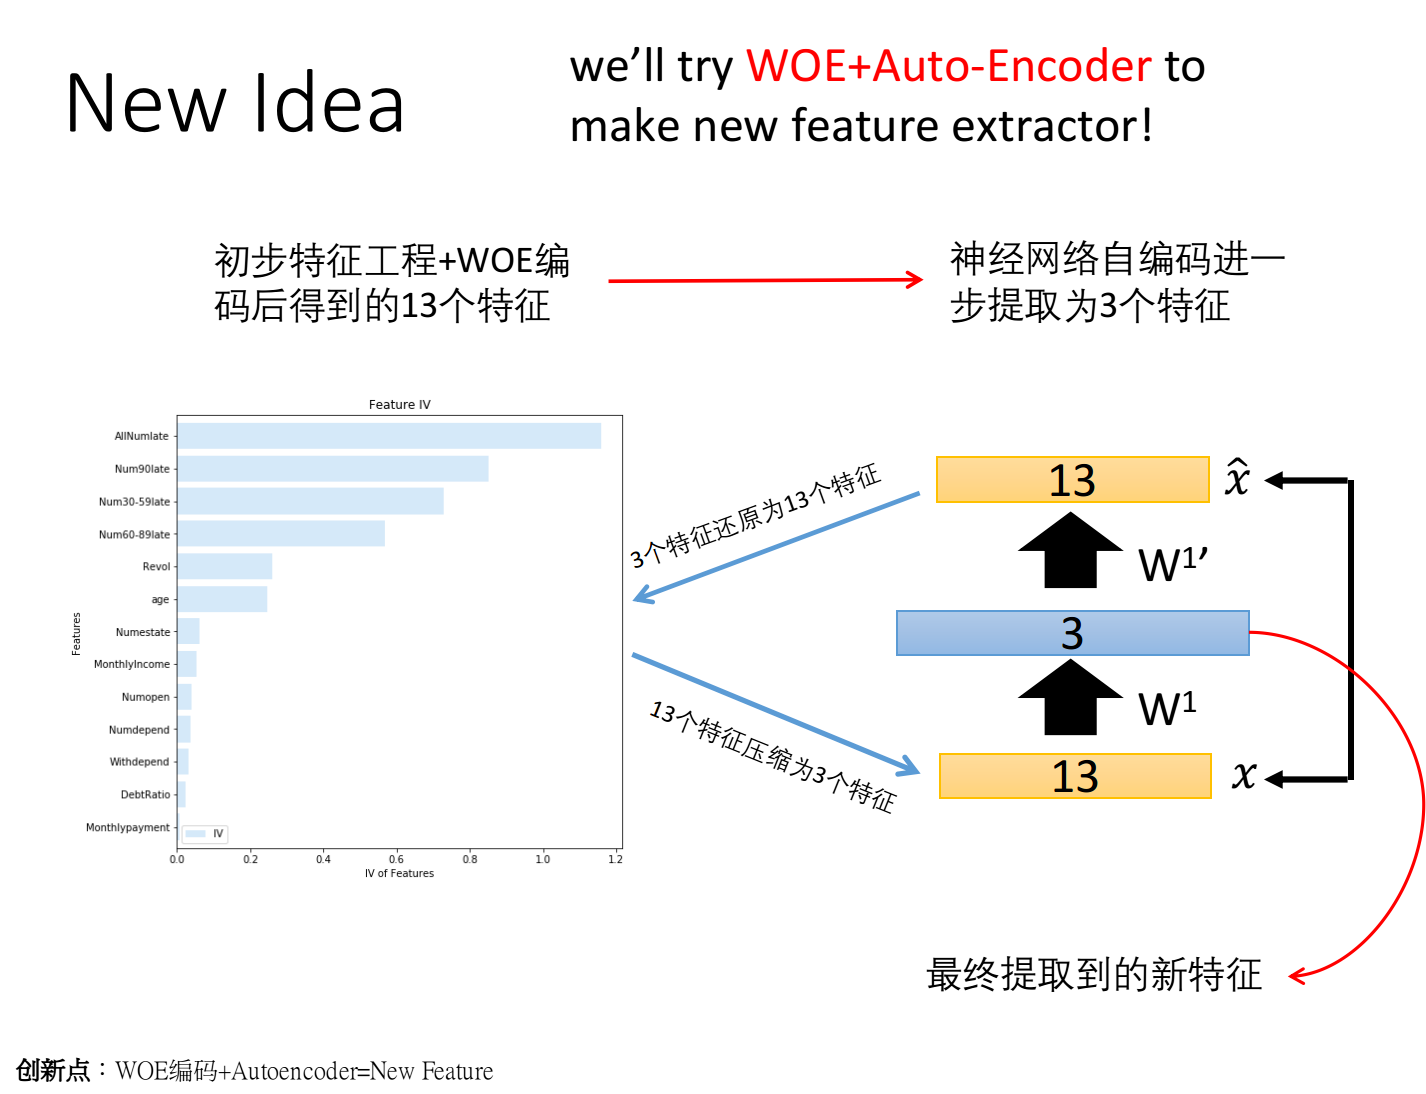
\includegraphics[width=0.7\linewidth]{idea.png}
    \caption{自编码模型简介}
    \label{fig:idea}
\end{figure}

\subsection{模型算法实现}
特征处理模型算法实现主要分为两部分,WOE编码和Auto-encoder特征提取。

\subsubsection{WOE编码}
实现数据分箱、WOE编码的关键算法如下,其中变量说明:

tar:target目标变量;var:进行woe,iv转换的自变量;n:分组数量。
\begin{lstlisting}[frame=shadowbox]
    def bin_woe(tar, var, n=None, cat=None):
    total_bad = tar.sum()
    total_good =tar.count()-total_bad
    totalRate = total_good/total_bad
    
    if cat == 's':
        msheet = pd.DataFrame({tar.name:tar,var.name:var,'var_bins':pd.qcut(var, n, duplicates='drop')})
        grouped = msheet.groupby(['var_bins'])
    elif (cat == 'd') and (n is None):
        msheet = pd.DataFrame({tar.name:tar,var.name:var})
        grouped = msheet.groupby([var.name])
        
    groupBad = grouped.sum()[tar.name]
    groupTotal = grouped.count()[tar.name]
    groupGood = groupTotal - groupBad
    groupRate = groupGood/groupBad
    groupBadRate = groupBad/groupTotal
    groupGoodRate = groupGood/groupTotal

    woe = np.log(groupRate/totalRate)
    iv = np.sum((groupGood/total_good-groupBad/total_bad)*woe)
    
    if cat == 's':
        new_var, cut = pd.qcut(var, n, duplicates='drop',retbins=True, labels=woe.tolist())
    elif cat == 'd':
        dictmap = {}
        for x in woe.index:
            dictmap[x] = woe[x]
        new_var, cut = var.map(dictmap), woe.index

    return woe.tolist(), iv, cut, new_var
\end{lstlisting}

\subsubsection{Auto-Encoder特征抽取模型}
PyTorch实现Auto-encoder自编码器的模型如下:
\begin{lstlisting}[frame=shadowbox]
    class AutoEncoder(nn.Module):
    def __init__(self):
        super(AutoEncoder, self).__init__()
        
        self.encoder = nn.Sequential(
            nn.Linear(13, 64),
            nn.Tanh(),
            nn.Linear(64, 32),
            nn.Tanh(),
            nn.Linear(32, 3)
        )
        
        self.decoder = nn.Sequential(
            nn.Linear(3, 32),
            nn.Tanh(),
            nn.Linear(32, 64),
            nn.Tanh(),
            nn.Linear(64, 13)
        )
        
    def forward(self, x):
        encode = self.encoder(x)
        decode = self.decoder(encode)
        return encode, decode
\end{lstlisting}

参数模型训练使用参数: EPOCH=100,lr=0.001,Loss=MSE,训练过程如下:
\begin{lstlisting}[frame=shadowbox]
    autoencoder = AutoEncoder()
    mse_loss = nn.MSELoss()
    optim = torch.optim.Adam(autoencoder.parameters(), lr=0.001)

    for epoch in range(100):
        for step, (x, _) in enumerate(train_loader):
            encode, decode = autoencoder(x)
            loss = mse_loss(decode, x)
            optim.zero_grad()
            loss.backward()
            optim.step()
            if step % 100 == 0:
                print('epoch_%d step_%d loss: %.4f' % (epoch, step, loss.data.item()))
\end{lstlisting}

\subsection{自编码结果可视化分析}
为了更直观地感受基于自编码降维的特征工程的效果,这里将降维后的三个维度可视化在三维空间上。下图是5万个样本点根据降维后的三个坐标绘制出来的图像,主要展示了两个方向上样本点的分布。

\begin{figure}[H]
    \centering
    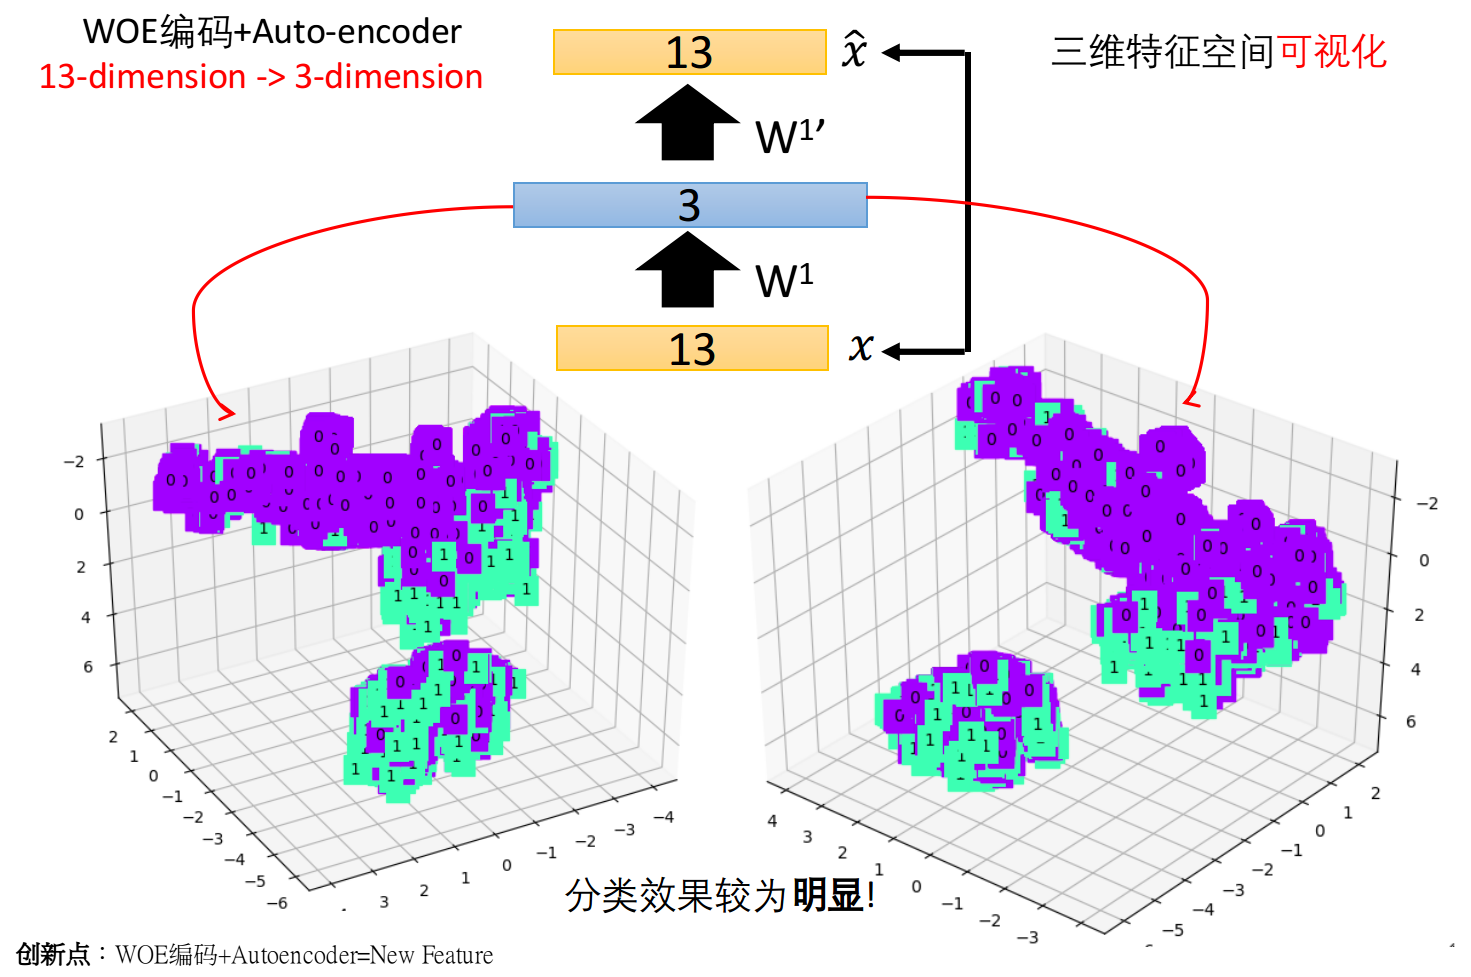
\includegraphics[width=0.7\linewidth]{visual.png}
    \caption{自编码特征结果可视化}
    \label{fig:visual}
\end{figure}

可以清楚地看到,通过该模型获取到的3-dimension feature具备较好的分类能力,能够使两个不同类别的样本点较为明显地分布在空间的两块不同区域。该实验结果表明,本文提出的方法确实具备一定的可行性,能够在一定程度上提高分类效果。\\

除了定性分析之外,接下来将定量对比分析“是否使用自编码提取特征”在相同分类模型上所表现出来的AUC值情况,来进一步证明该方法的正确性。

\subsection{不同分类器上的对比}
\subsubsection{简要说明}
这一节主要对比了,使用和未使用自编码特征提取的数据集在LightGBM、Random Forest、Logistic Regression上的表现,并测试了DNN作为分类器的表现。

\begin{itemize}
    \item 不使用自编码方法的数据集将根据前面的特征工程分析,通过woe、iv值筛选出清洗后的五个特征: “Num6089late”,“Num90late”,“AllNumlate”,“Revol”,“age”作为三个分类模型的输入,并观察分类效果和AUC值的表现。
    \item 使用自编码方法的数据集将初步数据清洗和WOE编码后的13维特征经过Autoencoder映射到3维,再作为四个分类模型的输入,观察分类效果和AUC值的表现。
\end{itemize}

\subsubsection{LightGBM模型上的表现对比}
为了方便对比,这里将两个数据集所使用的LightGBM参数设置为相同:

\begin{lstlisting}[frame=shadowbox]
    import lightgbm as lgb
    params = {
        'boosting_type': 'gbdt',
        'objective': 'binary',
        'metric': 'auc',
        'num_leaves': 15,
        'max_depth': -1,
        'min_data_in_leaf': 64,
        'learning_rate': 0.1,
        'feature_fraction': 0.8,
        'bagging_fraction': 0.8,
        'bagging_freq': 1,
        'verbose': -1,
        'is_unbalance': False,
        'num_boost_round': 200
    }
\end{lstlisting}

并同时建立了两个输入数据不同的分类器:

\begin{lstlisting}[frame=shadowbox]
    lgb_train = lgb.Dataset(X_train, Y_train)
    lgb_val = lgb.Dataset(X_validation, Y_validation)
    lgbm = lgb.train(params=params, train_set=lgb_train, valid_sets=lgb_val)  # classifier1
    ... # classifier2
\end{lstlisting}

两次实验的结果如下:\\

\begin{center}
    \begin{tabular}{ccc}
        \hline
                    & 普通特征工程 & 基于自编码降维的方法 \\
        \hline
        训练集(auc) & 0.8193       & 0.8489               \\
        \hline
        验证集(auc) & 0.8175       & 0.8271               \\
        \hline
    \end{tabular}
\end{center}

可以看到在LightGBM模型上,分类效果和AUC值都比较高,而相较于一般的特征工程,基于自编码降维的方法使得AUC值有了$1\%\sim\%3$的提升。\\

两次实验的roc曲线如下:
\begin{figure}[H]
    \centering
    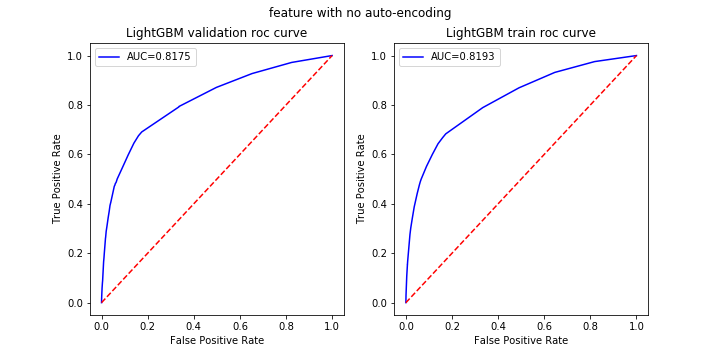
\includegraphics[width=0.8\linewidth]{lgbm_no.png}
    \caption{普通特征工程在LightGBM上的表现}
    \label{fig:lgbm_no}
\end{figure}

\begin{figure}[H]
    \centering
    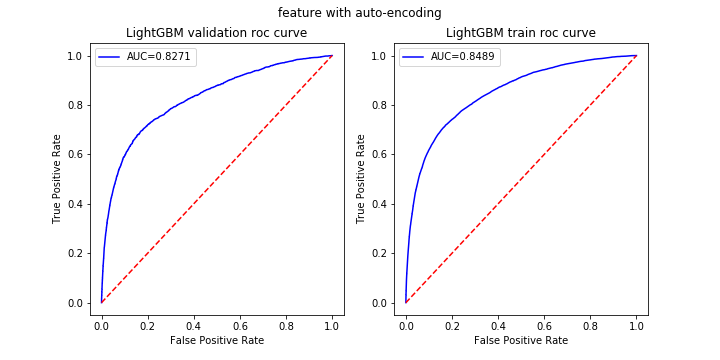
\includegraphics[width=0.8\linewidth]{lgbm.png}
    \caption{自编码在LightGBM上的表现}
    \label{fig:lgbm}
\end{figure}


\subsubsection{Random Forest模型上的表现对比}
同样的,设置两个随机森林模型的参数一致,去验证不同特征处理方法的数据集在相同分类模型上的表现。

\begin{lstlisting}[frame=shadowbox]
    from sklearn.ensemble import RandomForestClassifier

    for i in range(5, 10):
        for j in range(10, 20):
            rfc = RandomForestClassifier(n_estimators=j, max_depth=i, random_state=0)
            rfc.fit(X_train, Y_train)
            auc_train_rfc = roc_auc_score(Y_train, rfc.predict_proba(X_train)[:,1])
            auc_val_rfc = roc_auc_score(Y_validation, rfc.predict_proba(X_validation)[:,1])
            print("estimators: %d depth: %d\t auc_train: %.4f\t auc_validation: %.4f" % \
                (j, i, auc_train_rfc, auc_val_rfc))
\end{lstlisting}

两次实验的结果如下:\\

\begin{center}
    \begin{tabular}{ccc}
        \hline
                    & 普通特征工程 & 基于自编码降维的方法 \\
        \hline
        训练集(auc) & 0.8195       & 0.8433               \\
        \hline
        验证集(auc) & 0.8177       & 0.8255               \\
        \hline
    \end{tabular}
\end{center}

两次实验的roc曲线如下:
\begin{figure}[H]
    \centering
    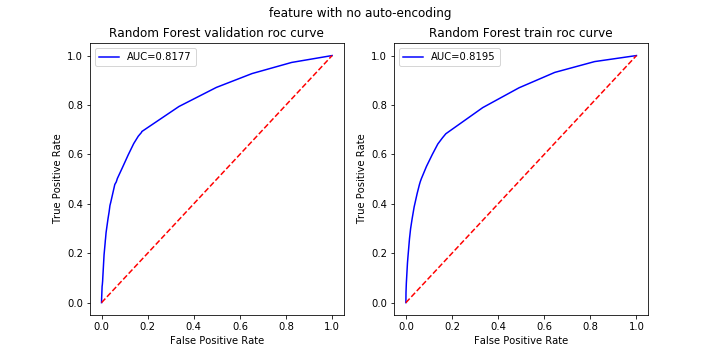
\includegraphics[width=0.8\linewidth]{rf_no.png}
    \caption{普通特征工程在Random Forest上的表现}
    \label{fig:rf_no}
\end{figure}

\begin{figure}[H]
    \centering
    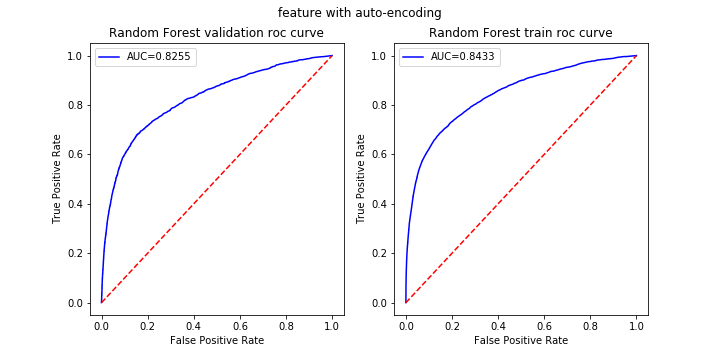
\includegraphics[width=0.8\linewidth]{rf_.png}
    \caption{自编码在Random Forest上的表现}
    \label{fig:rf}
\end{figure}

可以看到,相较于一般的特征工程,基于自编码降维的方法同样使得随机森林的AUC值有了$1\%\sim\%3$的提升。\\

\subsubsection{Logistic Regression模型上的表现对比}
除了树模型之外,这里还使用逻辑回归观察自编码降维的表现,实际上在之前的论述中已经提到,逻辑回归可以被看作是激活函数为sigmoid的网络层。

\begin{lstlisting}[frame=shadowbox]
    from sklearn.linear_model import LogisticRegression
    # LR_old ...
    LR_new=LogisticRegression(random_state=0,
                               solver="sag",
                               penalty="l2",
                               class_weight="balanced",
                               C=1.0,
                               max_iter=500)
    
    LR_new.fit(X_train_new, Y_train_new)
\end{lstlisting}

两次实验的结果如下:\\

\begin{center}
    \begin{tabular}{ccc}
        \hline
                    & 普通特征工程 & 基于自编码降维的方法 \\
        \hline
        训练集(auc) & 0.8182       & 0.7461               \\
        \hline
        验证集(auc) & 0.8177       & 0.7529               \\
        \hline
    \end{tabular}
\end{center}

两次实验的roc曲线如下:
\begin{figure}[H]
    \centering
    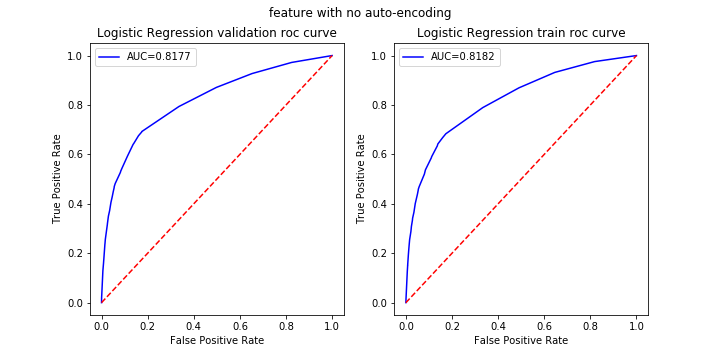
\includegraphics[width=0.8\linewidth]{lr_no.png}
    \caption{普通特征工程在Logistic Regression上的表现}
    \label{fig:rf_no}
\end{figure}

\begin{figure}[H]
    \centering
    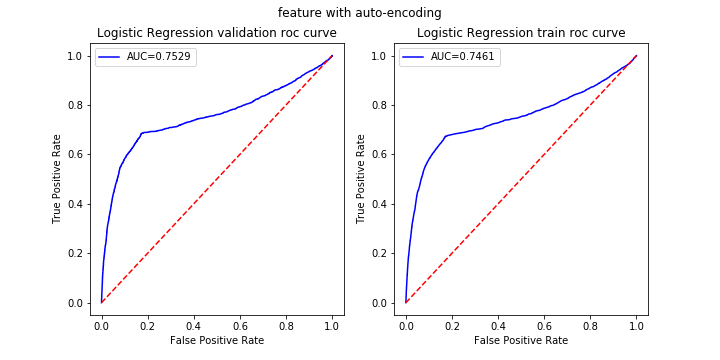
\includegraphics[width=0.8\linewidth]{lr.png}
    \caption{自编码在Logistic Regression上的表现}
    \label{fig:rf}
\end{figure}

可以看到,如果把逻辑回归当做网络层来看,它的分类能力甚至不如一般的隐藏层来得好,这也就导致了最终AUC表现反而有所下降。

\subsubsection{Neural Network上的表现}
这里特地设计了把整个神经网络作为分类器的实验内容,既是为了和逻辑回归进行对比,表明逻辑回归的分类能力不如一般的隐藏层好;又是为了和树模型进行对比,表明神经网络自编码提取到的特征+树模型得到的分类效果会比纯粹的神经网络分类器要好。\\

神经网络模型如下:
\begin{lstlisting}[frame=shadowbox]
    class CreditClassifier(nn.Module):
        def __init__(self):
            super(CreditClassifier, self).__init__()
            self.layer1 = nn.Linear(3, 32)
            self.layer2 = nn.Linear(32, 16)
            self.layer3 = nn.Linear(16, 1)
            
        def forward(self, x):
            x = torch.relu(self.layer1(x))
            x = torch.relu(self.layer2(x))
            x = torch.sigmoid(self.layer3(x))
            return x
\end{lstlisting}

实验的结果如下:

\begin{center}
    \begin{tabular}{ccc}
        \hline
         & 训练集(auc) & 验证集(auc) \\
        \hline
         & 0.8270      & 0.8238      \\
        \hline
    \end{tabular}
\end{center}

实验的roc曲线如下:
\begin{figure}[H]
    \centering
    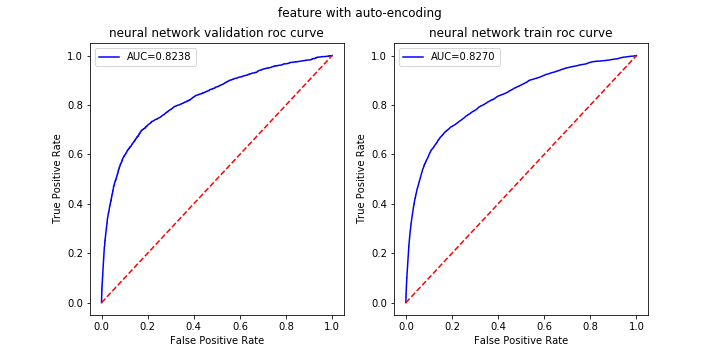
\includegraphics[width=0.8\linewidth]{nn_.png}
    \caption{Neural Network上的表现}
    \label{fig:nn}
\end{figure}

上图中可以看出,神经网络分类器确实优于逻辑回归,但又劣于自编码加树模型的表现。
\subsection{评分卡的制作}
标准评分卡采用的格式是评分卡中的每一个变量都遵循一系列IF-THEN法则。数据记录中每一个变量的值都适用此法则的结果决定了该特定变量所分配的分支,总分就是评分卡中所有变量的贡献的和。
此处仅用传统特征工程+LR分类器得到的结果进行评分卡的制作,作为示例。本文其他模型的评分卡制作同理。\cite{ref5} \\
评分卡制作过程如下:
\begin{lstlisting}[frame=shadowbox]
	intercept=LR.intercept_
	coef=LR.coef_
	coe=coef[0].tolist()
	coe_df=pd.DataFrame({'feature':IV_info,'coe':coe})

	import math
	B=20/math.log(2)
	A=600+B*math.log(1/20)
	#basic score
	score=round(A-B*intercept[0],0)

	featurelist = []
	woelist = []
	cutlist = []
	for k,v in woe_dict.items():
	if k in IV_info:
	for n in range(0,len(v)):
	featurelist.append(k)
	woelist.append(v[n])
	cutlist.append(cut_dict[k][n])
	scoreboard = pd.DataFrame({'feature':featurelist,'woe':woelist,'cut':cutlist},
	columns=['feature','cut','woe'])
	score_df=pd.merge(scoreboard,coe_df)
	score_df['score']=round(-B*score_df['woe']*score_df['coe'],0)
	score_df.drop('coe',axis=1,inplace=True)
	score_df
\end{lstlisting}
得到评分卡:
\begin{figure}[H]
	\centering
	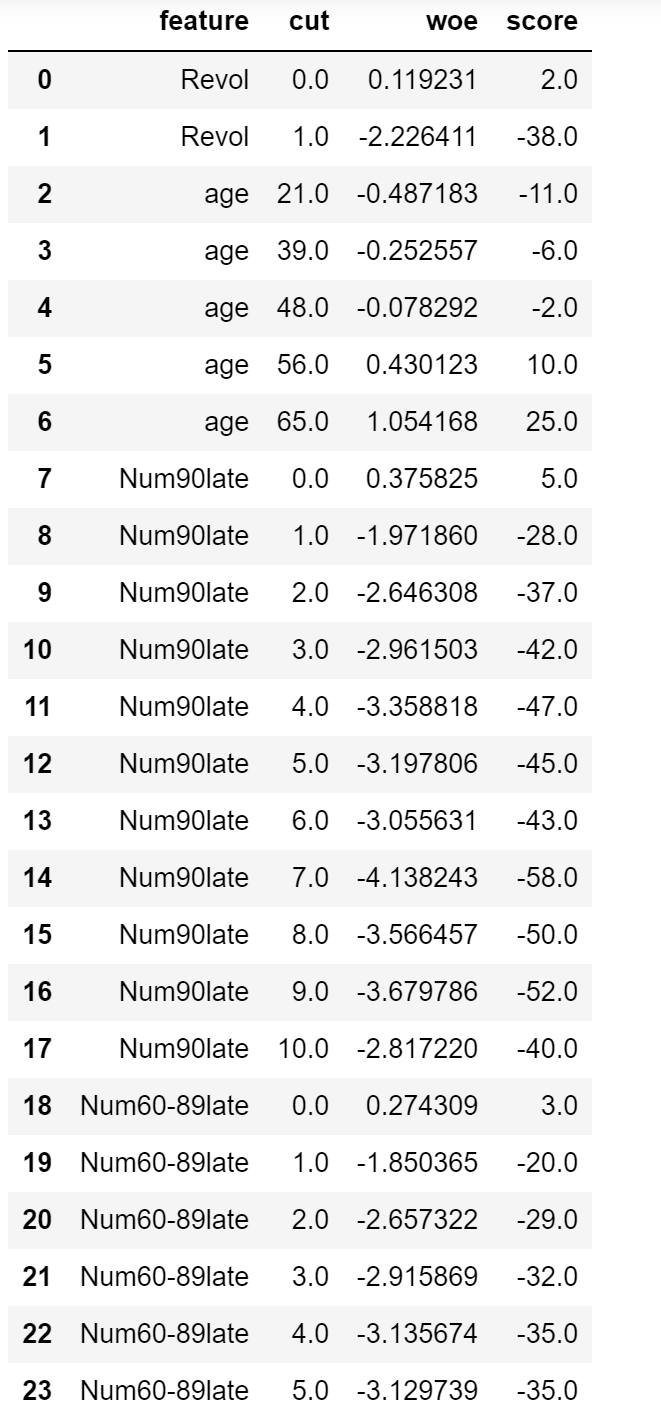
\includegraphics[width=0.4\linewidth]{score.png}
	\caption{评分卡}
\end{figure}

\subsection{实验总结与分析}

下面对所有实验的模型表现做一个总结,以验证本文提出的基于自编码降维的方法在风控领域的实际应用能力:\\

\begin{center}
    \begin{tabular}{lll}
        \hline
        采用的模型                                & 训练集(auc) & 验证集(auc) \\
        \hline
        LightGBM(普通特征工程)                    & 0.8193      & 0.8175      \\
        \hline
        Random Forest(普通特征工程)               & 0.8195      & 0.8177      \\
        \hline
        Logistic Regression(普通特征工程)         & 0.8182      & 0.8177      \\
        \hline
        LightGBM(基于自编码降维的方法)            & 0.8489      & 0.8271      \\
        \hline
        Random Forest(基于自编码降维的方法)       & 0.8433      & 0.8255      \\
        \hline
        Logistic Regression(基于自编码降维的方法) & 0.7461      & 0.7529      \\
        \hline
        Neural Ntework Classifier(神经网络分类器) & 0.8270      & 0.8238      \\
        \hline
    \end{tabular}
\end{center}


可以看到,基于自编码降维的方法+树模型分类器(random forest, lightgbm等)得到的auc值和分类效果普遍优于同等条件下使用普通特征工程的结果,都能够得到$1\%\sim3\%$的提升,可见本文提出的方法在树模型上具备一定的应用价值。\\

此外,传统的神经网络方法、普通特征工程后的逻辑回归、基于自编码后的逻辑回归,auc值和分类效果依次下降。经过分析,如果把逻辑回归当做网络层,那么它的分类能力反而不如可以选择其他激活函数的级联隐藏层,因此传统神经网络要优于逻辑回归,而自编码后的特征分布,更适合树模型的决策过程,而并不符合逻辑回归的特性,因此自编码后的逻辑回归性能反而有$3\%\sim4\%$的下降。\\

综合分析可知,基于自编码降维的方法+LightGBM模型在该数据集上的表现最好。

\newpage
\section{结论与展望}
本文创新地提出了自编码降维模块,其提取的3D特征比起传统特征工程在大部分分类器上都能有更优的性能。一方面,该模块的使用能一定程度上提升auc值;另一方面,比起手工进行特征的提取,自编码降维显然具有更高的稳定性和可靠性。其中,基于自编码降维的方法+LightGBM模型在该数据集上的表现最好。\\

由此可见,从整体上而言,利用Auto-encoder神经网络进行特征转换和提取在大数据风控的场景中是比较适用的。\\

当然,尽管如此,算法优化的幅度并不是十分显著。在LightGBM, Random Forest等分类器上,预测结果的auc值只得到$1\%\sim3\%$的提升。这带给我们更多关于如何更好在大数据风控领域应用好自适应编码模型的思考。\\

首先,本文将降维获得的特征固定为三维。这意味着数据集的信息会遭受一定程度上的丢失。后续实验可以尝试更多的可能维数k,探究k与auc值的关系。在未来,还可以尝试把自编码模块的神经网络由DNN改进为CNN或者其他模型。\\

在本场景、本数据集中,自编码降维模块体现了一个尚佳的水平,但并不意味着对于所有的风控场景和数据集来说,它的性能都能够得到保持。另一方面,本文的自编码降维模块的对比仅局限于一个传统特征工程,无法说明它能始终优于传统特征工程的平均水平。本文采取的分类器也局限于LightGBM, Random Forest, Logistic Regression, Neural Network Classifier,无法代表将其应用于所有监督学习模型的结果。在未来,应该在更多的更复杂和全面的测试集上增加对比测试,并且需要在相同条件下分析各个算法的优势和弊端,整合算法亮点,探索出一种准确性、稳定性等等方面都表现优异的算法。\\

关于信用评分系统的实践在本篇报告中告一段落,但之后持续的优化和完善工作并不会停止。或许金融科技领域的知识和技能挖掘也如同此次的实践一样,等待研究者们用充足的热情、持久的耐心以及不懈的毅力去践行。


% -------------------------------------------------------------------
% Appendices
% -------------------------------------------------------------------

% \begin{appendices}
%     \input{sections/appendix.tex}
% \end{appendices}

\newpage
\end{document}